\documentclass[10pt]{article}

% ---------------------------------------------------------------- layout (NeurIPS-like preprint)
\usepackage[letterpaper,textwidth=5.5in,textheight=9in,top=1in,headsep=0.25in,footskip=0.4in]{geometry}
\usepackage[T1]{fontenc}
\usepackage{newtxtext,newtxmath}
\usepackage{microtype}
\usepackage{graphicx}
\usepackage{booktabs}
\usepackage{multirow}
\usepackage{array}
\usepackage{tabularx}
\usepackage{amsmath}
\usepackage{bm}
\usepackage[dvipsnames]{xcolor}
\usepackage{enumitem}
\usepackage[font=small,labelfont=bf,skip=4pt]{caption}
\usepackage{subcaption}
\usepackage[round,sort&compress]{natbib}
\usepackage{algorithm}
\usepackage{algpseudocode}
\usepackage{fancyhdr}
\usepackage[colorlinks=true,linkcolor=RoyalBlue,citecolor=RoyalBlue,urlcolor=RoyalBlue]{hyperref}
\usepackage{url}

\setlist{itemsep=1pt,topsep=3pt,leftmargin=1.4em}
\setlength{\parskip}{3pt}
\setlength{\parindent}{0pt}
\renewcommand{\arraystretch}{1.12}

\pagestyle{fancy}
\fancyhf{}
\renewcommand{\headrulewidth}{0pt}
\fancyfoot[C]{\thepage}
\fancypagestyle{first}{\fancyhf{}\fancyfoot[L]{\small Preprint. Work in progress; numbers are from pilot runs (one training seed per arm). 27 October 2026.}}

\newcommand{\genesis}{\textsc{Genesis}}
\newcommand{\aff}[1]{\textsf{\small[affordance]}~#1}
\newcommand{\dpay}{deaths\,/\,agent-yr}
\newcommand{\status}[1]{\textsf{\footnotesize #1}}

\title{\bfseries \genesis{}: A Homeostatic-Reward-Only Artificial Ecology\\for Studying What Social Structure Can Emerge,\\with First Results from Recurrent PPO Agents}

\author{%
  Advik Divekar \qquad Heet Ranpura\\[2pt]
  \small \genesis{} project\\
  \small \url{https://github.com/HeetRanpura/Genesis}
}
\date{}

\begin{document}
\maketitle
\thispagestyle{first}

% =====================================================================================================
\begin{abstract}
Most multi-agent reinforcement learning (MARL) studies of cooperation build part of the answer into the reward:
team rewards, prosocial bonuses, influence terms or communication losses. Under those designs it is hard to say
whether a social behaviour \emph{emerged} or was \emph{specified}. We present \genesis{}, a seeded, procedurally
generated foraging ecology in which every agent is rewarded \emph{only} for keeping its own body near a physiological
setpoint (homeostatic reinforcement learning), plus a death penalty. The rule is enforced by a unit test. Ecological
features that make social behaviour possible or useful, but never rewarding, are documented as \emph{affordances}:
large prey that need two simultaneous hunters, food that can be carried and dropped, scarce fresh water, and seasonal
winters. Every cognitive or social capacity is a configuration switch that is off by default. The engine is a fused
Numba kernel. It simulates a $256\times256$ world with 1{,}000 agents, three species of food-limited scripted fauna,
weather, fire and floods at $\approx$112k steps per minute including observations, on a laptop CPU. Runs are
bit-reproducible, and every agent at every tick is recorded and exactly replayable. We pair the engine with a
preregistered evaluation protocol: training on worlds 1000+, evaluation on held-out worlds 0--4, three non-learning
baselines in every comparison, and bootstrap confidence intervals with Hedges' $g$.

In a first study, parameter-shared recurrent (GRU) and memoryless PPO agents trained for 19.7M agent-steps reach
1.80 and 1.58 \dpay{} on held-out worlds. Both clearly beat random (3.83) and greedy (3.31) foragers but cannot be
distinguished from a hand-written heuristic (1.50). Decomposing mortality shows why. The learners nearly eliminate
thirst, predator and fire deaths (thirst 0.09 vs.\ 0.96 \dpay{} for the heuristic), but die of starvation, mostly
in winter. Over the first half-year (spring--summer) their mortality is 4--6$\times$ lower than the heuristic's
(0.19 and 0.33 vs.\ 1.22). In winter it is 1.4--1.9$\times$ higher. A first-order energy budget computed from the
recorded event stream shows that the learners' intake ($1.31$--$1.34\times10^{-3}$ per tick, 73--74\% from plants)
barely covers basal metabolism ($1.3\times10^{-3}$). The memoryless agent survives better largely because it moves
less and rests more (48\% of winter actions vs.\ 23\% for the GRU agent). Memory reduced thirst deaths 2.7-fold but
did not reduce all-cause mortality at this budget. Learners also persist in futile behaviour: 78--91\% of their
\textsc{drink} actions during droughts happen with no water in reach, against 30--37\% otherwise. We report these
results as pilots, with all negative results kept. We describe the measurement framework, null models and
preregistered replication (3 seeds per arm, in progress) that will test whether any social organisation appears
at all. Applying the preregistered internal-state and social analyses to the pilot checkpoints, we find four things.
Linear probes decode own hydration, energy and predator presence from the GRU state ($R^2$ 0.70 and 0.85; AUC 0.91). The
value estimate predicts death within 200 ticks (AUC 0.98). The GRU state carries no more information about out-of-view
water than the network's current encoding does. Learners cluster more than water and habitat explain, but blinding them
to other agents leaves the clustering intact, so it is not social. We found no cooperative large-prey hunting.
\end{abstract}

% =====================================================================================================
\section{Introduction}
\label{sec:intro}

Human social life (sharing food, hunting together, signalling, keeping traditions, enforcing norms) appears in the
archaeological and ethnographic record in a rough order, under particular ecological conditions
\citep{tomasello1999cultural,tennie2009ratchet}. A computational testbed could probe the \emph{structural} side of
this question. Given learners that care only about their own bodies, and an ecology in which cooperation is possible
and sometimes useful, which social regularities appear, in what order, and under which conditions? We are explicit
about the scope of the analogy. Our agents are small neural policies, not models of early humans, and any comparison
we eventually draw is between orders of emergence and triggering conditions, not between minds.

\paragraph{The confound we want to remove.}
Much MARL research on cooperation adds social terms to the objective. Examples are inequity aversion
\citep{hughes2018inequity}, social-influence bonuses \citep{jaques2019influence}, shared team rewards, or
differentiable communication channels trained end to end \citep{foerster2016communicate}. These are excellent tools
for \emph{engineering} cooperation. When the question is whether cooperation \emph{emerges}, they make the answer
partly true by construction. Benchmarks such as Melting Pot \citep{leibo2021meltingpot} and sequential social
dilemmas \citep{leibo2017ssd} instead fix a game and ask how well agents play it. Large persistent worlds such as
Neural MMO \citep{suarez2019neuralmmo} provide scale and competition but are not built around physiological need.
Artificial-life systems such as Tierra and PolyWorld \citep{ray1991tierra,yaeger1994polyworld} pioneered open-ended
ecologies, mostly without modern deep RL learners or preregistered statistics.

\paragraph{Our approach.}
\genesis{} combines four commitments:
\begin{enumerate}
\item \textbf{Reward purity.} Each agent's reward is the reduction of its own homeostatic drive, following
\citet{keramati2014homeostatic}, plus a death penalty. The reward has no social term, shaping or curiosity bonus.
A unit test fails if the reward ever depends on anything but the agent's own body.
\item \textbf{Affordances, not incentives.} Every ecological feature that could make social behaviour useful
(cooperatively hunted large prey, droppable food, a kin-similarity cue, optional huddling warmth) is tagged and
switchable, so its effect can be ablated.
\item \textbf{Capabilities as switches.} Memory, world models, communication, social learning, reputation, niche
construction, reproduction and aggression are all off by default. Experiments turn on exactly one thing at a time.
\item \textbf{Evaluation discipline.} Agents train and are evaluated on disjoint world seeds. Three non-learning
baselines appear in every comparison. Hypotheses and decision rules are preregistered before evaluation
\citep{nosek2018preregistration}, and uncertainty is reported over seeds
\citep{henderson2018matters,agarwal2021precipice}.
\end{enumerate}

\begin{figure}[t]
\centering
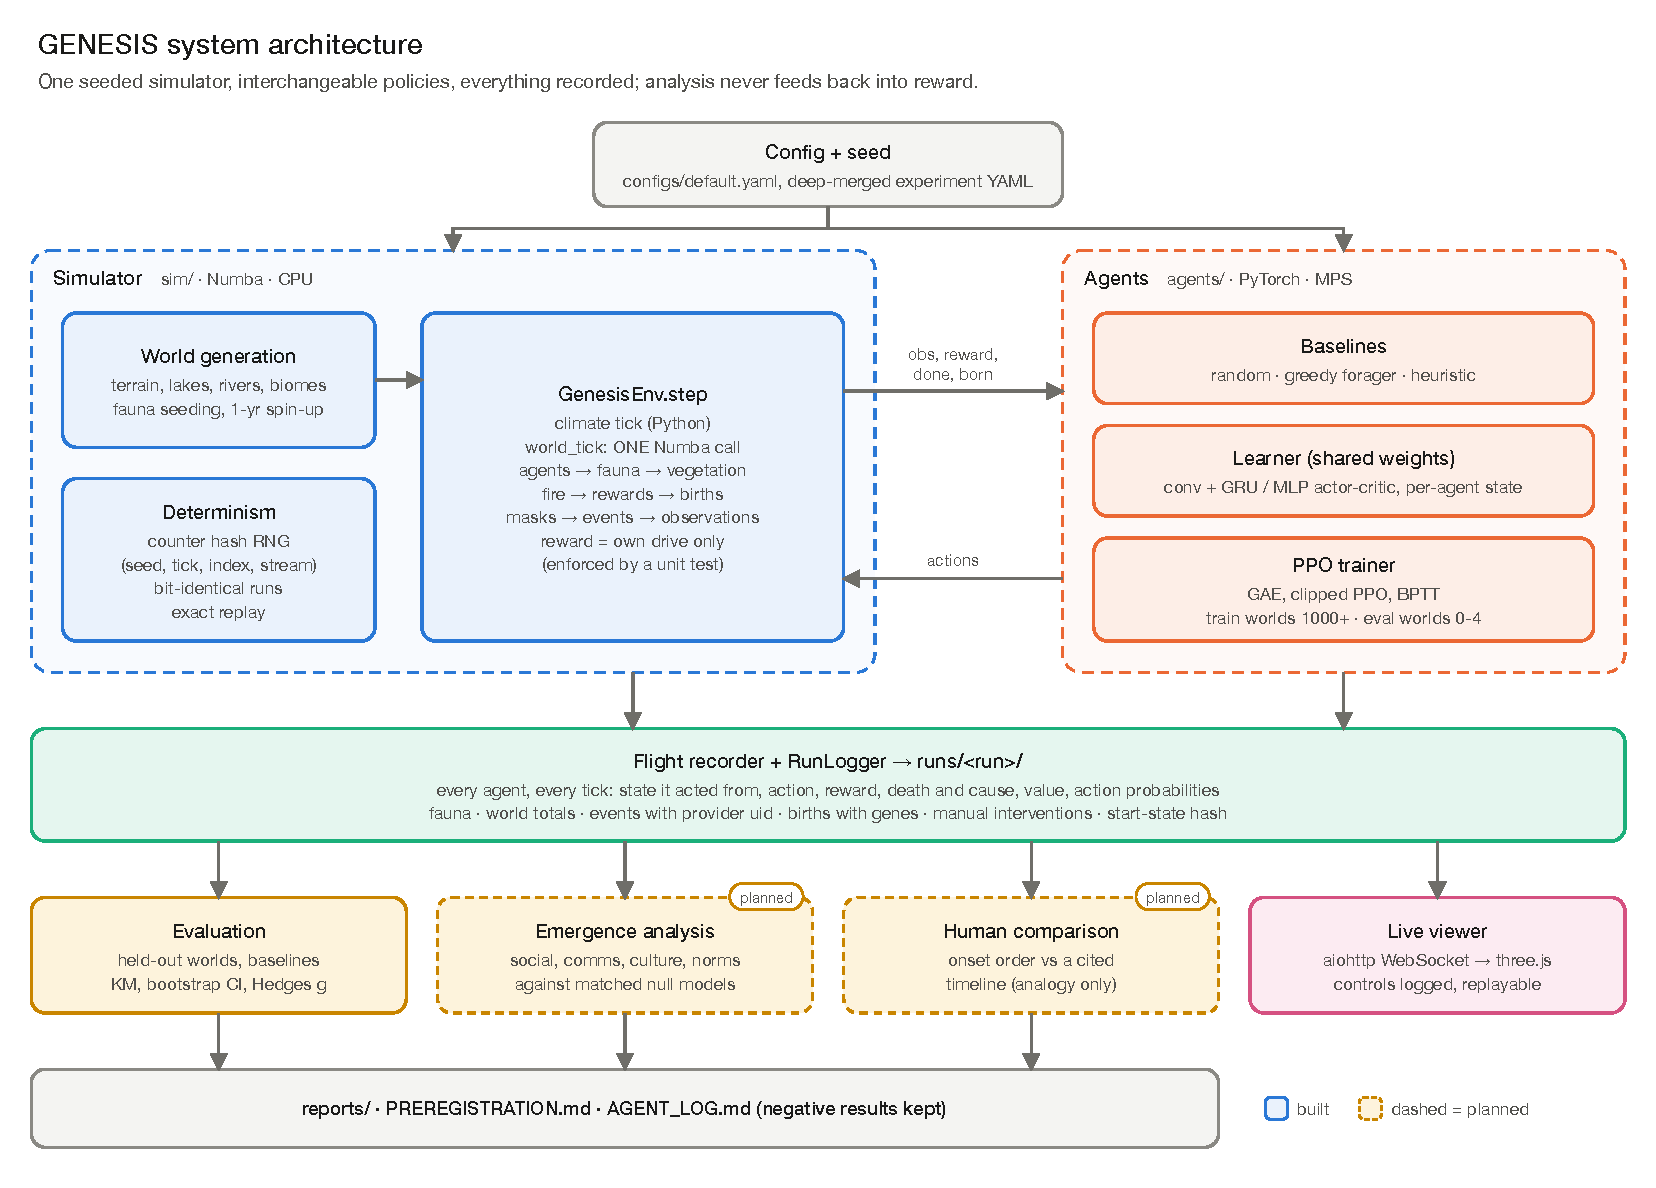
\includegraphics[width=\linewidth]{diagrams/01_system_architecture.pdf}
\caption{\textbf{System architecture.} A seeded simulator and interchangeable policies exchange observations and actions; a flight recorder captures every agent at every tick. Evaluation, emergence analysis and the viewer only read the recordings, so nothing downstream can feed back into the reward. Dashed boxes are planned.}
\label{fig:arch}
\end{figure}

Fig.~\ref{fig:arch} gives the overall architecture.

\paragraph{Contributions.}
\begin{itemize}
\item \textbf{An engine} (\S\ref{sec:world}). A deterministic, food-limited, seasonal ecology with 1{,}000+ agents at
$\approx$112k steps/min with observations on a laptop CPU. It has a counter-based RNG, so results do not depend on the
thread count, an incrementally maintained observation image, precomputed line-of-sight masks, and a flight recorder
that makes every run exactly replayable.
\item \textbf{A protocol} (\S\ref{sec:protocol}). Held-out worlds, baselines, preregistration, a strict
non-overlap rule for ``beats'', and explicit units of replication.
\item \textbf{First learner results} (\S\ref{sec:results}). Survival-only PPO agents beat random and greedy foragers
but not a hand-written heuristic. A season-resolved, cause-resolved and energy-resolved analysis attributes the gap
to a winter energy deficit. Memory trades thirst deaths for starvation deaths, and learned policies remain inflexible
when the environment changes (droughts). Probes, value calibration, null models and a causal ``social blinding''
ablation separate genuine social structure from look-alikes (\S\ref{sec:h6h7}).
\item \textbf{A measurement framework} (\S\ref{sec:measure}). Operational definitions, null models and planted-truth
unit tests for social, communicative and cultural phenomena, preregistered before any of them is measured.
\end{itemize}

We stress what we do \emph{not} claim. No social behaviour has yet been measured with the Stage-3 instruments, and we
expect none in the capability-off setting reported here (preregistered H4/H7).

% =====================================================================================================
\section{Related work}
\label{sec:related}

\paragraph{Homeostatic and need-based RL.}
\citet{keramati2014homeostatic} showed that rewarding the reduction of a drive, defined as a distance from a
physiological setpoint, makes reward seeking and physiological stability the same objective. They also derived
temporal discounting as a pressure toward the shortest path to the setpoint. We adopt their drive-reduction reward
verbatim over four variables: energy, hydration, health and warmth.

\paragraph{Emergent cooperation and social learning in MARL.}
Sequential social dilemmas \citep{leibo2017ssd} and the Melting Pot suite \citep{leibo2021meltingpot} evaluate
cooperation and generalisation to new co-players. Emergent tool use \citep{baker2020tooluse}, bartering
\citep{johanson2022bartering} and social learning \citep{ndousse2021social,bhoopchand2023cultural} show that rich
behaviour can arise from simple objectives when the environment supports it. \citet{ndousse2021social} in particular
found that independent model-free agents rarely learn from experts without auxiliary losses. This is a warning for
our capability-off agents. Parameter-shared PPO is a strong default in cooperative MARL \citep{yu2022mappo}.

\paragraph{Emergent communication.}
Agents can learn referential signalling games \citep{lazaridou2017emergence} and differentiable channels
\citep{foerster2016communicate}. \citet{lowe2019pitfalls} showed that common metrics can mislead, and recommend
measuring both positive signalling and positive listening, with causal tests. We adopt their distinction.

\paragraph{Artificial life and evolution.}
Tierra \citep{ray1991tierra} and PolyWorld \citep{yaeger1994polyworld} pioneered open-ended ecologies. The Baldwin
effect \citep{hinton1987baldwin} motivates our planned learning-plus-evolution experiments.

\paragraph{Continual learning.}
Our agents live in a non-stationary world (seasons, disturbances, new worlds). Catastrophic forgetting
\citep{kirkpatrick2017ewc} and loss of plasticity \citep{dohare2024plasticity} are therefore first-class concerns,
not afterthoughts.

\paragraph{Cultural evolution.}
We operationalise traditions following the exclusion method of \citet{whiten1999cultures}, the cumulative ratchet
following \citet{tennie2009ratchet}, and communication properties following Hockett's design features
\citep{hockett1960origin}.

% =====================================================================================================
\section{The \genesis{} world}
\label{sec:world}

\begin{figure}[t]
\centering
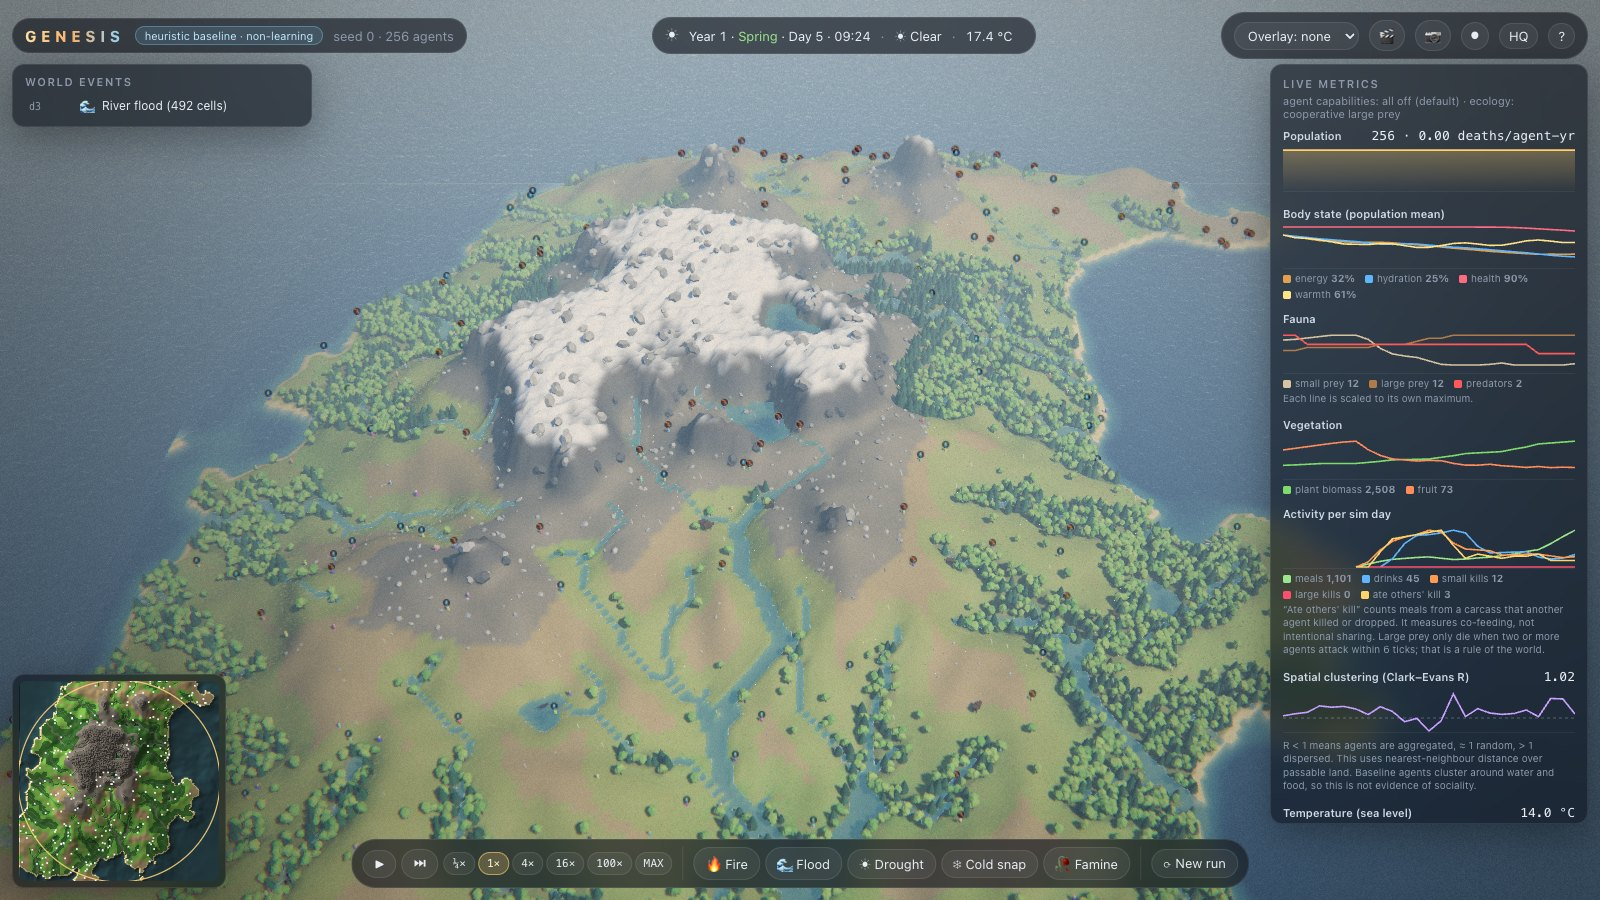
\includegraphics[width=\linewidth]{assets/02_overview.jpg}
\caption{\textbf{The live viewer on held-out world 0} (three.js; \S\ref{app:viewer}). Agents (dots) forage across
forest, grassland and river networks around a central mountain massif. The right panel shows live, measured
quantities: population, mean body state, fauna, vegetation, activity and the Clark--Evans aggregation index.
Terrain relief and foliage are visual only. Everything on the dashboard is computed from simulator state.}
\label{fig:teaser}
\end{figure}

\subsection{Time, terrain and water}
One tick is one action per agent. A day is 120 ticks, a season 8 days, and a year 3{,}840 ticks: spring, summer,
autumn, winter. Every run begins with one simulated year of ecology without agents (\emph{spin-up}), so the lush
initial state's boom and crash is not part of the experiment.

The world (default $256\times256$) is generated from the seed in these steps:
\begin{enumerate}
\item domain-warped fractal elevation with a continental falloff, then rank normalisation;
\item priority-flood depression filling \citep{barnes2014priority}, which turns filled depressions into lakes;
\item D8 flow accumulation \citep{ocallaghan1984extraction}: rivers at $\geq$180 upstream cells, streams at $\geq$90;
\item a moisture field;
\item biomes: deep and shallow water, sand, grass, meadow, forest, barren, rock, mountain and caves.
\end{enumerate}
The ocean is \emph{salt}. Fresh water comes only from rivers, streams and lakes, which cover about 4--6\% of the
map (Fig.~\ref{fig:worlds}). Water is therefore spatially scarce and often out of view. That is what can make memory
useful.

\begin{figure}[t]
\centering
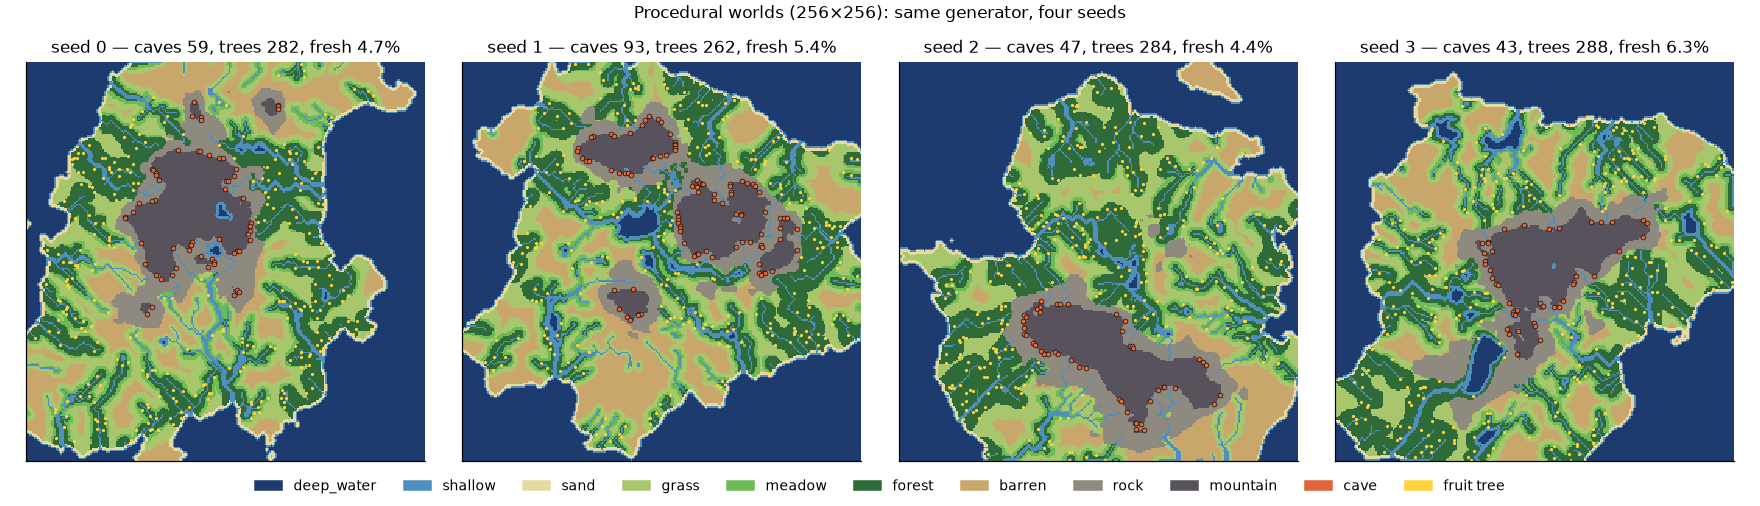
\includegraphics[width=\linewidth]{assets/fig1_terrain_seeds.png}
\caption{\textbf{Procedural worlds from four seeds.} Fresh water covers 4.4--6.3\% of the land. Caves (red) are
shelter; fruit trees are yellow. Seeds 0--4 are reserved for evaluation and never used in training.}
\label{fig:worlds}
\end{figure}

\subsection{Resources and fauna}
\paragraph{Plants.}
Plants regrow logistically toward a per-cell fertility. Growth is scaled by season (spring 1.2, summer 1.0,
autumn 0.55, winter 0.05), by rain ($+25\%$), drought ($\times0.4$), famine ($\times0.25$) and temperature (none below
2\,$^\circ$C). A grazed cell regrows from a 10\% floor (roots). One \textsc{eat} bite removes 0.25 biomass, worth at
most 0.03 energy.

\paragraph{Fruit trees.}
Each tree fruits in one season (up to 6 fruit at 0.15 energy each).

\paragraph{Carcasses.}
Carcasses spoil linearly. Each carcass remembers the uid of whoever killed or dropped it, so every meal records its
provider, which is what the sharing analysis needs.

\paragraph{Fauna.}
The three animal species are scripted, because they are part of the environment, and \emph{food-limited}: each
animal has an energy store, a metabolism (torpor at $\times0.2$ below 5\,$^\circ$C), grazing satiation, and seasonal
births from a full store.
\begin{itemize}
\item \textbf{Small prey} flee within 4 cells. One hunter suffices: a kill succeeds with probability 0.6 and leaves
0.30 energy.
\item \textbf{Large prey} also browse woody forage in forests. Without this niche, small prey competitively exclude
them.
\item \textbf{Predators} hunt agents and prey within 8 cells and never enter caves.
\end{itemize}
Population caps and immigration floors exist only as safety rails. Over 5 seeds $\times$ 3 years the caps never bind
(0\% of time), and the floors bind rarely. The exception is predators, which sit at their floor about 31\% of the
time when 256 heuristic agents compete with them for small prey. We report this as a known weakness.

\subsection{Weather and disturbances}
A daily Markov chain drives rain, fog (view radius 3), summer droughts (streams dry up; plant growth $\times0.4$;
fire risk $\times4$), winter cold snaps ($-10$\,$^\circ$C) and famine years. Wildfires ignite daily with a small
probability, spread by fuel and dryness, are put out by rain and leave burn scars. Spring floods turn floodplains into
shallow water. Snow builds up where it rains below 0\,$^\circ$C. All disturbances can also be triggered manually; every
trigger is logged with all its parameters and replayed exactly (Fig.~\ref{fig:timeline}).

\begin{figure}[t]
\centering
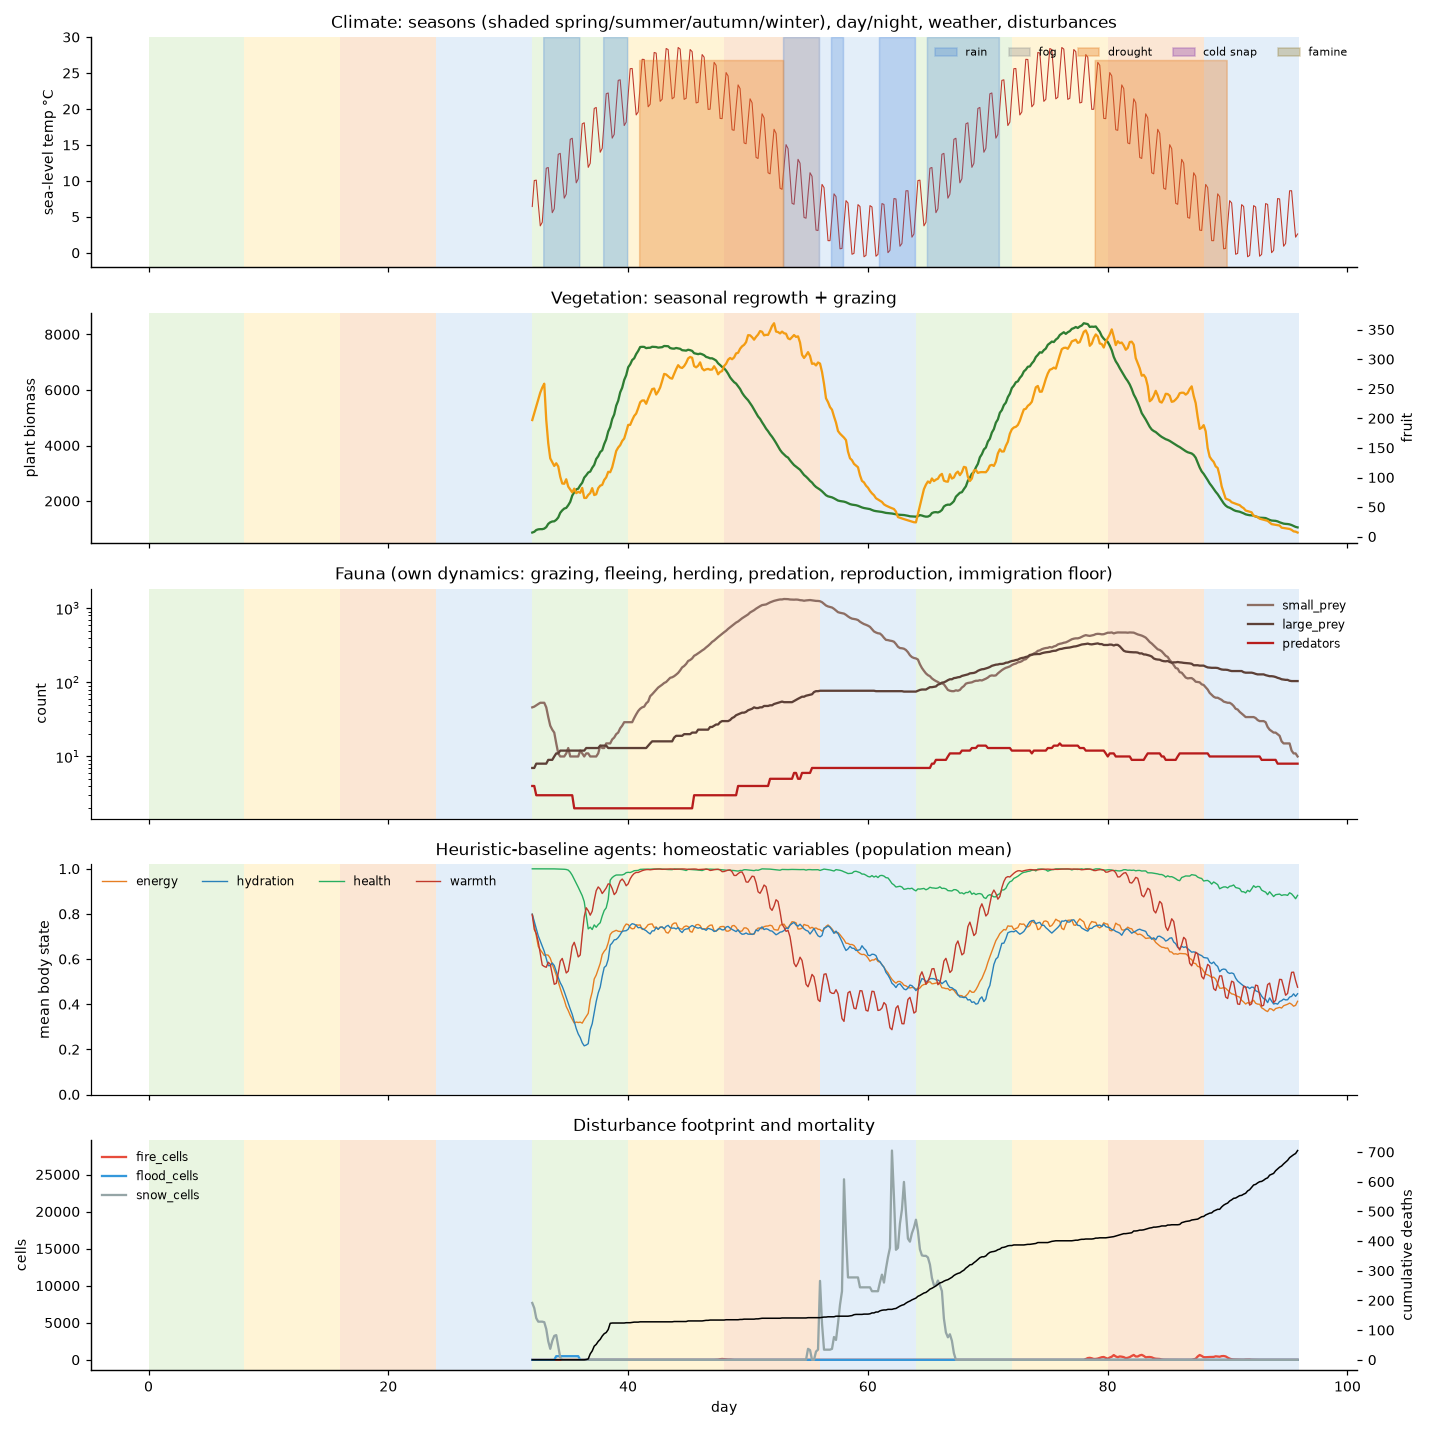
\includegraphics[width=\linewidth]{assets/fig3_timeline.png}
\caption{\textbf{Two years of one world} (seed 0, heuristic agents). From top: sea-level temperature with weather and
disturbance episodes; plant biomass and fruit; food-limited fauna (log scale); population-mean body state; disturbance
footprint and cumulative deaths. Shading marks the seasons. Spin-up (the first 32 days) is excluded from all statistics.}
\label{fig:timeline}
\end{figure}

\subsection{Agents: body, perception, actions}
\paragraph{Body.}
Each agent's body has four homeostatic variables $\bm h=(e,w,\eta,\theta)\in[0,1]^4$: energy, hydration, health and
warmth. It also has an age, and a heritable lifespan of 3--4 years. Energy falls by a basal cost of $1.3\times10^{-3}$
per tick, halved while resting and scaled by body size, plus $9\times10^{-4}$ per move, scaled by terrain
($\times1.25$ forest, $\times1.6$ rock, $\times2$ shallow water, more in snow), plus a carrying cost.
\begin{itemize}
\item \textbf{Hydration} falls by $1.6\times10^{-3}$ per tick ($\times2$ above 31\,$^\circ$C, $\times0.7$ while
resting).
\item \textbf{Warmth} relaxes toward a target set by the effective temperature, which depends on altitude, shelter,
forest, rain, snow and resting.
\item \textbf{Health} falls when energy or hydration hits zero, when warmth is below 0.2, and from fire, predators,
large-prey kicks or strikes. It regenerates when all needs are met.
\end{itemize}

\paragraph{Genes.}
Eight floats: lifespan, body size, cold tolerance and five neutral markers. The markers drive appearance and the
\aff{kin-similarity} cue.

\paragraph{Perception.}
\begin{itemize}
\item \textbf{Grid view.} An egocentric $11\times11\times16$ uint8 grid (Fig.~\ref{fig:obs}). The 16 channels are:
visible, blocked, water, forest, rock, shelter, plant, fruit, food item, small prey, large prey, predator, agent
(value encodes genetic similarity), fire, signal and snow.
\item \textbf{Occlusion.} Line of sight is blocked by mountains and by a second forest cell. The view radius shrinks
from 5 to 2 at night and to 3 in fog.
\item \textbf{Vector inputs.} A 13-feature interoceptive self-vector, up to 4 visible neighbours (9 features each),
and heard signals (used only when communication is on).
\end{itemize}

\paragraph{Actions.}
There are 11 base actions: noop, move N/E/S/W, rest, eat, drink, hunt, pickup and drop. Switches add build,
strike and $n_{\text{sym}}$ signal actions.
\begin{itemize}
\item \textbf{Drink} succeeds only next to fresh water or floodwater, or anywhere while it rains (a small amount).
\item \textbf{Food transfer.} Pickup and drop are always available, so food can be carried and dropped where another
agent can take it. This is the \aff{food-transfer} affordance.
\end{itemize}

\begin{figure}[t]
\centering
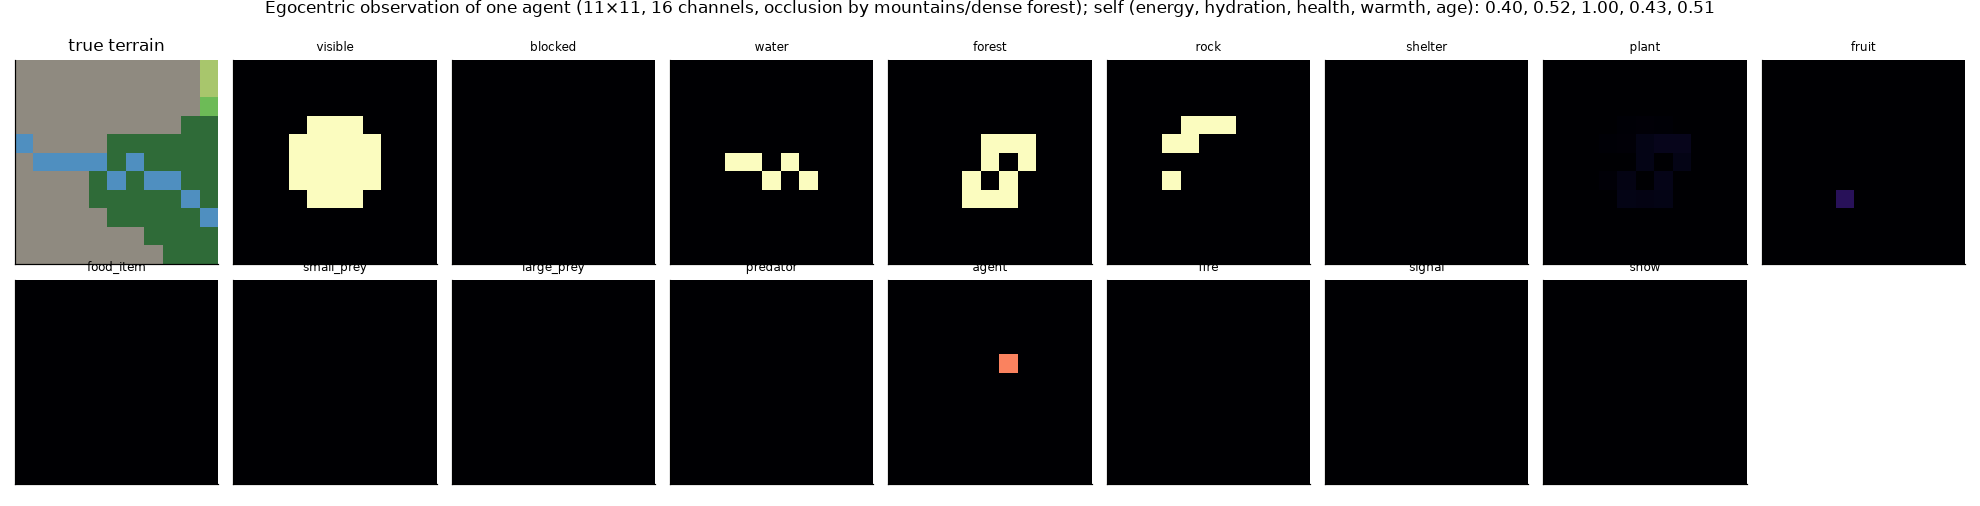
\includegraphics[width=\linewidth]{assets/fig7_observation.png}
\caption{\textbf{One agent's observation.} True terrain (left) and the 16 egocentric channels after line-of-sight
masking. Two forest cells or a mountain block sight. The agent sees only the bright disc in ``visible''.}
\label{fig:obs}
\end{figure}

\subsection{Reward (the hard rule)}
With setpoint $\bm h^\ast=(1,1,1,0.8)$, the drive is
\begin{equation}
D(\bm h)=\big\lVert \max(\bm h^\ast-\bm h,\,0)\big\rVert_2,
\end{equation}
and the reward is
\begin{equation}
r_t = D(\bm h_t)-D(\bm h_{t+1}) + c_{\text{death}}\,\mathbb 1[\text{died}_t] \;\big(+\,c_{\text{repro}}\,\mathbb 1[\text{reproduced}_t]\big),
\label{eq:reward}
\end{equation}
with $c_{\text{death}}=-1$ and $c_{\text{repro}}=0$ by default. Eq.~\ref{eq:reward} depends only on the agent's own
body. The test \path{test_reward_is_own_homeostatic_drive_only} recomputes Eq.~\ref{eq:reward} from each agent's
body state alone over 200 random-action ticks and asserts that it equals the environment's reward exactly.

\begin{figure}[t]
\centering
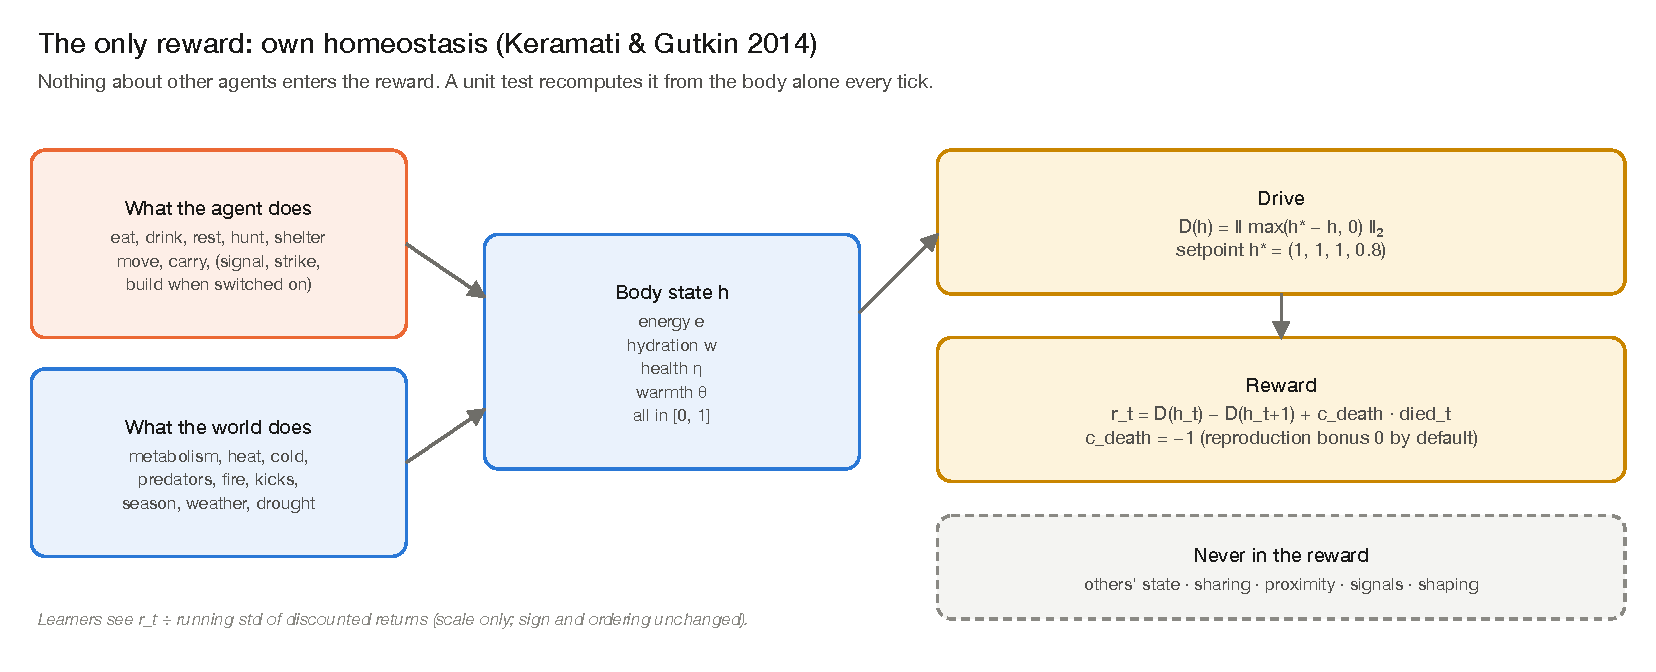
\includegraphics[width=0.92\linewidth]{diagrams/09_homeostatic_reward.pdf}
\caption{\textbf{The reward.} Actions and the world change the body; the reward is the reduction of the agent's own drive plus a death penalty. Nothing about other agents enters it.}
\label{fig:reward}
\end{figure}

\subsection{Affordances and capability switches}
Table~\ref{tab:switches} lists every switch. Affordances make social behaviour \emph{possible or useful}; nothing
makes it \emph{rewarding}. In the experiments reported here, all capabilities are off and only cooperative large prey
is on.

\begin{table}[t]
\centering\small
\caption{\textbf{Switches.} Affordances (A) change the ecology; capabilities (C) change what agents can do or
perceive. Defaults are in the right column.}
\label{tab:switches}
\begin{tabularx}{\linewidth}{@{}l c X c@{}}
\toprule
Switch & Type & Effect & Default\\
\midrule
\texttt{cooperative\_large\_prey} & A & large-prey kill needs $\geq2$ distinct attackers within 6 ticks; carcass 1.8 energy & on\\
\texttt{huddle\_warmth} & A & each adjacent agent adds $+1.5\,^\circ$C (biases aggregation) & off\\
food pickup/drop & A & food can be carried and left for others; provider logged & always\\
agent channel value & A & encodes genetic similarity of visible agents (kin cue) & always\\
\midrule
\texttt{memory} & C & recurrent core (GRU) in the policy & off\\
\texttt{world\_model} & C & latent dynamics model and imagination (planned) & off\\
\texttt{communication} & C & $n_{\text{sym}}{=}8$ costly signals, heard within 9 cells & off\\
\texttt{social\_learning} & C & neighbours' last actions visible & off\\
\texttt{reputation} & C & neighbours' share/strike histories visible & off\\
\texttt{aggression} & C & \textsc{strike} action (makes punishment possible) & off\\
\texttt{niche\_construction} & C & wood/stone pickup, \textsc{build} shelters & off\\
\texttt{reproduction} & C & births with mutated heritable genes; no respawn & off\\
\bottomrule
\end{tabularx}
\end{table}

\subsection{Engine design and performance}
\label{sec:engine}
One tick is a Python climate update followed by \emph{one} Numba \citep{lam2015numba} call, \texttt{world\_tick}. It
runs agents, fauna, vegetation and trees, fire, rewards, births and respawns, reward masks, event tally and
observations in order. Figs.~\ref{fig:worldgen}--\ref{fig:obspipe} (Appendix) detail generation, the tick and observations.
Three design choices make it fast and exact:
\begin{enumerate}
\item \textbf{Counter-based RNG.} All in-kernel randomness is a SplitMix-style hash of
(seed, tick, index, stream) \citep{steele2014splitmix,salmon2011random}. Parallel loops draw no shared state, and
sequential resolution follows hash-derived permutations. A run is therefore a pure function of (config, seed,
actions), whatever the thread count.
\item \textbf{Incremental observation image.} Observations are masked crops of a world image $I[y,x,16]$ that is
patched in place at every mutation site, not rebuilt every tick. A test compares it with a full rebuild.
\item \textbf{Static line of sight.} Terrain never changes, so each cell's line-of-sight mask is precomputed once by
propagation along Bresenham parent chains.
\end{enumerate}
Table~\ref{tab:bench} reports throughput. A PettingZoo \texttt{ParallelEnv} wrapper \citep{terry2021pettingzoo}
passes the official API test.

\begin{table}[t]
\centering\small
\caption{\textbf{Engine throughput} (median of interleaved runs; Apple M4 laptop CPU, fanless, so absolute numbers
are conservative). ``Obs'' includes building every agent's observation.}
\label{tab:bench}
\begin{tabular}{@{}rrcrr@{}}
\toprule
World & Agents & Obs & Steps/min & Agent-steps/s\\
\midrule
$256^2$ & 256 & no & 211{,}287 & 0.90M\\
$256^2$ & 256 & yes & 146{,}188 & 0.62M\\
$256^2$ & 1{,}000 & no & 171{,}568 & 2.86M\\
$256^2$ & 1{,}000 & yes & \textbf{111{,}992} & \textbf{1.87M}\\
$256^2$ & 2{,}000 & yes & 89{,}041 & 2.97M\\
$512^2$ & 1{,}000 & yes & 59{,}499 & 0.99M\\
\bottomrule
\end{tabular}
\end{table}

% =====================================================================================================
\section{Agents and training}
\label{sec:agents}

\subsection{Baselines}
Three non-learning policies act on exactly the observations learners receive. None has a social rule.
\begin{itemize}
\item \textbf{Random} acts uniformly over the actions.
\item \textbf{Greedy forager} attends to its lower of energy and hydration. It eats or drinks if possible, otherwise
walks to the nearest visible resource for that need, otherwise explores.
\item \textbf{Heuristic} follows hand-written survival rules. It flees predators and fire. It drinks below hydration
0.55 until 0.95 and eats below energy 0.6 until 0.9 (with hysteresis). It also hunts adjacent small prey, seeks
shelter when cold and rests at night when sated.
\end{itemize}

\subsection{Learner}
\paragraph{Architecture.}
All agents share one actor-critic (about 1.1M parameters), and each keeps its own recurrent state.
\begin{itemize}
\item \textbf{Grid branch:} conv$3{\times}3$(32), then conv$3{\times}3$ stride 2 (64), then FC 256.
\item \textbf{Vector branch:} FC 64 over the self, neighbour and signal inputs.
\item \textbf{Trunk and heads:} the two branches are concatenated, passed through FC 256 and then the core, then
policy and value heads.
\item \textbf{Core:} \texttt{GRUCell}(256) \citep{cho2014gru} in the \emph{GRU} arm; a 256-unit feed-forward layer in
the \emph{memoryless} arm, otherwise identical.
\end{itemize}
A slot's hidden state is zeroed when a new agent occupies it.

\paragraph{Learning rule.}
Clipped PPO \citep{schulman2017ppo} with GAE \citep{schulman2016gae}. Fig.~\ref{fig:net} shows the network, and
Fig.~\ref{fig:loop}, Algorithm~\ref{alg:train} and Table~\ref{tab:hparams} give the loop and hyper-parameters.
\begin{itemize}
\item Each of the 256 slots is a continuing experience stream.
\item A death cuts the bootstrap, because the slot's next observation belongs to a newborn.
\item The GRU arm is trained by back-propagation through the whole 128-tick rollout, starting from the hidden state
stored at rollout time.
\end{itemize}
The training world changes every 40 iterations (seeds $1000, 1001, \dots$), so agents see seasons, droughts and new
maps. The network runs on Apple MPS and the world on CPU.

\begin{figure}[t]
\centering
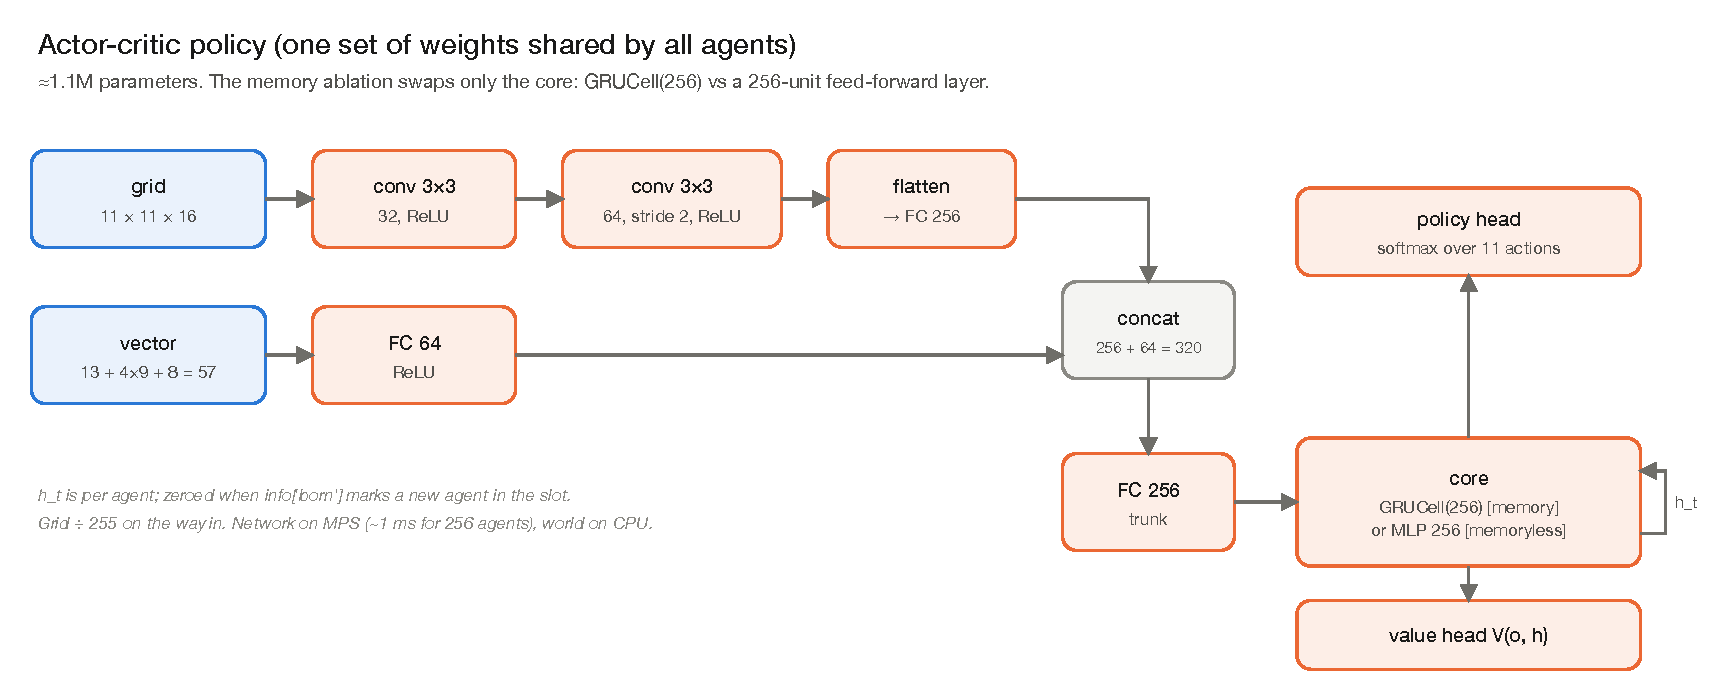
\includegraphics[width=\linewidth]{diagrams/05_policy_network.pdf}
\caption{\textbf{Policy network.} One set of weights is shared by all agents; each agent has its own recurrent state. The memoryless arm replaces only the GRU core.}
\label{fig:net}
\end{figure}

\begin{figure}[t]
\centering
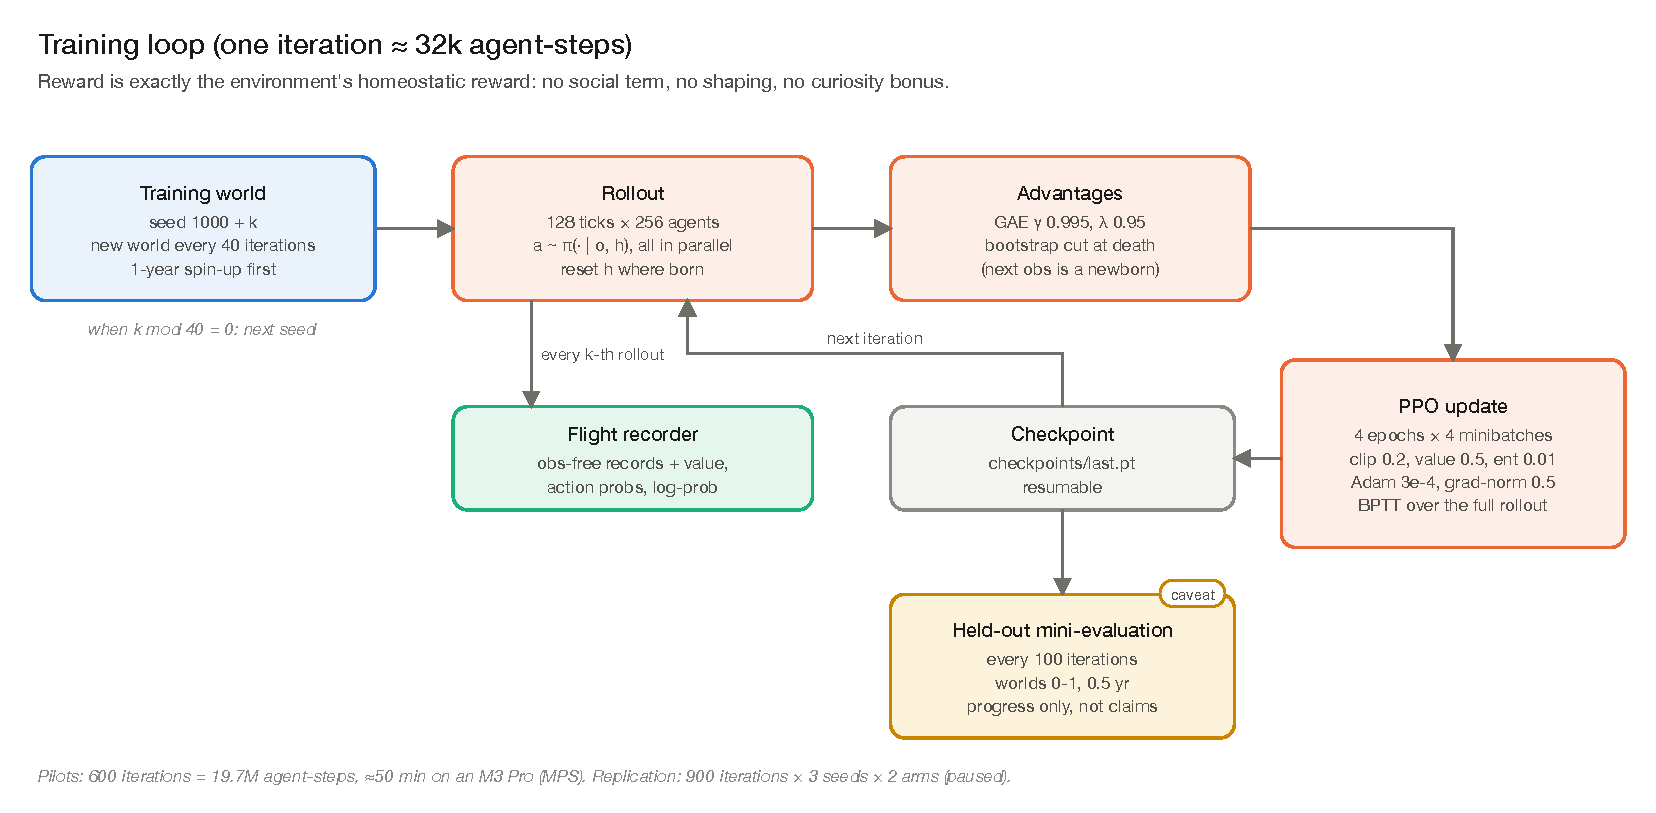
\includegraphics[width=\linewidth]{diagrams/06_training_loop.pdf}
\caption{\textbf{Training loop.} Each iteration collects 128 ticks from 256 agents, computes GAE advantages with the bootstrap cut at deaths, and runs a clipped-PPO update. Held-out mini-evaluations use a half-year horizon and track progress only (see Fig.~\ref{fig:horizon}).}
\label{fig:loop}
\end{figure}

\begin{algorithm}[t]
\caption{Training loop of the pilots (original \texttt{agents/rppo.py}, since folded into \texttt{agents/ppo.py} with the same defaults)}
\label{alg:train}
\begin{algorithmic}[1]
\State world $\gets$ \textsc{Generate}(seed $=1000$); spin up 1 year; spawn 256 agents
\For{iteration $k=0,\dots,K-1$}
  \If{$k \bmod 40 = 0$ and $k>0$} world $\gets$ \textsc{Generate}(seed $=1000+k/40$) \EndIf
  \For{$t=1..128$} \Comment{rollout, all agents in parallel}
     \State $a_t \sim \pi_\phi(\cdot\mid o_t, h_t)$; \quad $(o_{t+1}, r_t, d_t, \text{born}_t) \gets$ \textsc{WorldTick}$(a_t)$
     \State $h_{t+1}[\text{born}_t] \gets 0$; \quad record $(o_t,a_t,\log\pi,V,r_t,d_t)$ to the flight recorder
  \EndFor
  \State $\hat A \gets$ GAE$(\gamma{=}0.995,\lambda{=}0.95)$, bootstrap cut at deaths
  \For{4 epochs $\times$ 4 minibatches over agents} \Comment{full-sequence BPTT}
     \State minimise $-L^{\text{clip}}(\epsilon{=}0.2) + 0.5\,L^{V} - 0.01\,\mathcal H[\pi]$; clip $\lVert\nabla\rVert\le0.5$
  \EndFor
  \If{$k \bmod 100 = 0$} held-out mini-evaluation (worlds 0--1, 0.5 yr) \EndIf
\EndFor
\end{algorithmic}
\end{algorithm}

\begin{table}[t]
\centering\small
\caption{\textbf{Learner hyper-parameters} (identical across arms except the core).}
\label{tab:hparams}
\begin{tabular}{@{}ll@{\hspace{2em}}ll@{}}
\toprule
Rollout & 128 ticks $\times$ 256 agents & Discount $\gamma$ / GAE $\lambda$ & 0.995 / 0.95\\
Iterations (pilot) & 600 (19.7M agent-steps) & PPO clip $\epsilon$ & 0.2\\
Epochs $\times$ minibatches & $4\times4$ & Learning rate (Adam) & $3\times10^{-4}$\\
Value coef.\ / entropy coef. & 0.5 / 0.01 & Gradient-norm clip & 0.5\\
Hidden size & 256 & World switch & every 40 iterations\\
Device & Apple MPS (M3 Pro) & Wall time per run & $\approx$50 min\\
\bottomrule
\end{tabular}
\end{table}

% =====================================================================================================
\section{Evaluation protocol and preregistration}
\label{sec:protocol}

\paragraph{Protocol.}
Every policy (learner or baseline) is run on held-out worlds 0--4 for 2 simulated years with 256 agents and a fixed
population (a dead agent's slot is refilled at a random land cell). Actions are sampled, not taken greedily.

\paragraph{Lifetimes.}
Lifetimes are measured from the end of spin-up. An earlier version measured them from tick 0, which halved measured
mortality; that bug is fixed and covered by a regression test.

\paragraph{Metrics.}
\begin{itemize}
\item mortality (deaths per agent-year lived);
\item Kaplan--Meier survival at one year \citep{kaplan1958nonparametric};
\item median lifetime;
\item cause-specific death rates;
\item per-season mortality and energy reserves.
\end{itemize}

\paragraph{Statistics.}
The unit of replication in the pilot is the evaluation world ($n=5$). We report the mean and a 95\% percentile
bootstrap CI over worlds \citep{efron1979bootstrap}, plus Hedges' $g$ \citep{hedges1981distribution}. ``A beats
B'' means the two CIs do not overlap; overlapping CIs are reported as ``not distinguishable at $n=5$'', never as a
win.

\begin{figure}[t]
\centering
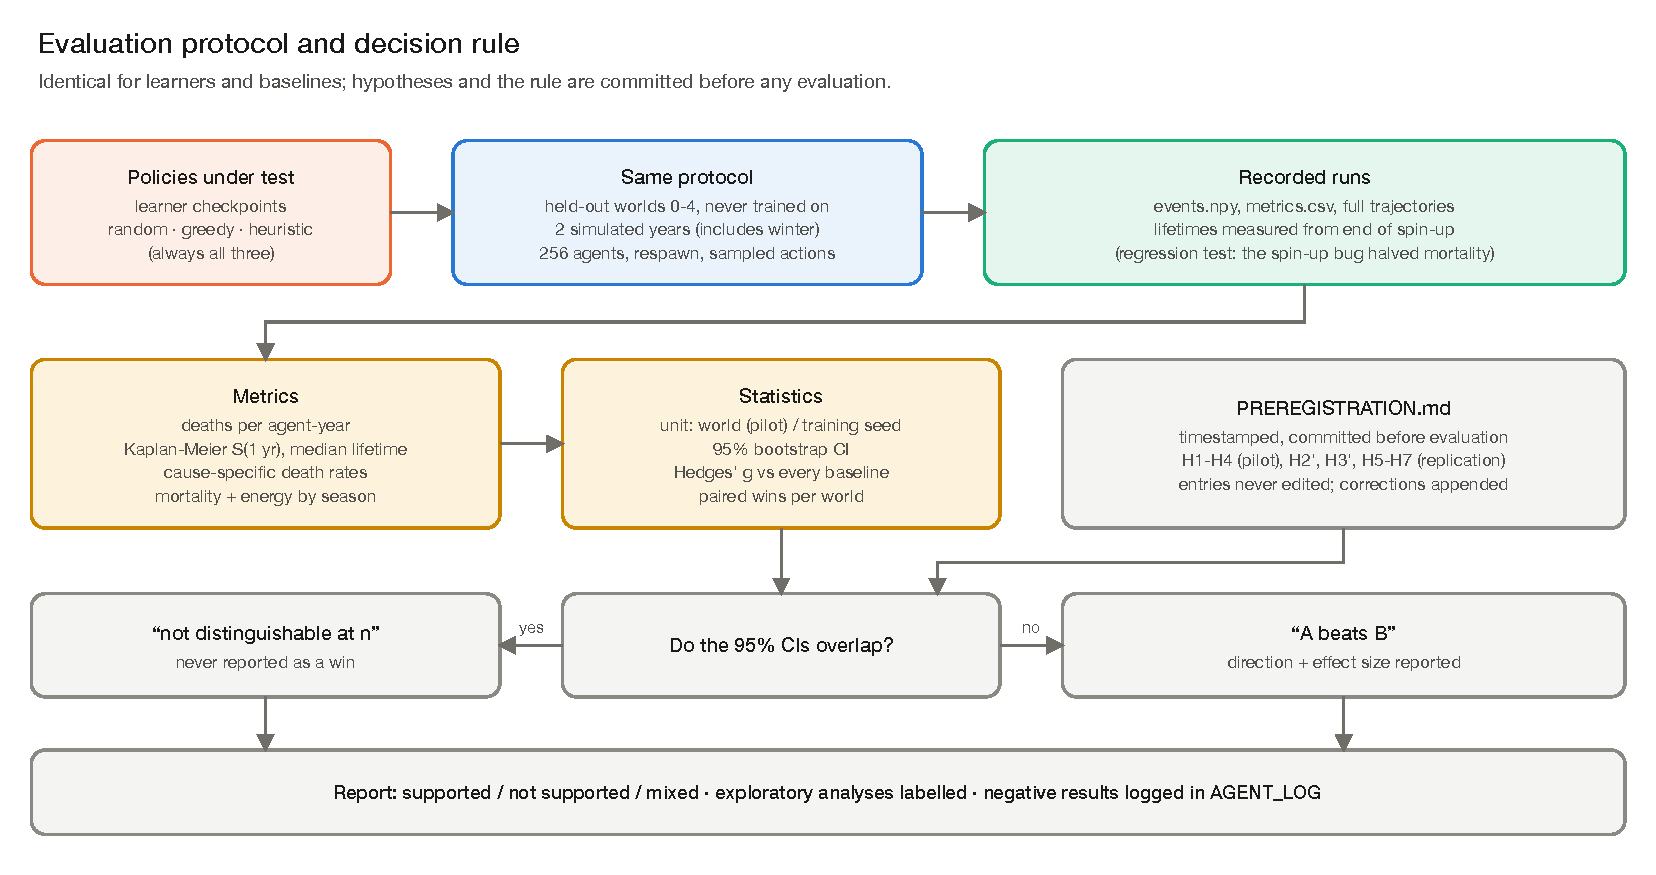
\includegraphics[width=\linewidth]{diagrams/07_evaluation_protocol.pdf}
\caption{\textbf{Evaluation protocol and decision rule.} Learners and baselines run the same protocol on held-out worlds. ``Beats'' requires non-overlapping 95\% CIs; the hypotheses and the rule are committed before evaluation.}
\label{fig:eval}
\end{figure}

\paragraph{Preregistration.}
Hypotheses H1--H4 were committed to \texttt{docs/PREREGISTRATION.md} at 21:20 IST on 26 Oct 2026, before any
evaluation:
\begin{itemize}
\item \textbf{H1:} the GRU learner beats random and greedy.
\item \textbf{H2:} the GRU learner beats the heuristic.
\item \textbf{H3:} the GRU learner has fewer thirst deaths than the memoryless learner, with all-cause mortality no
higher.
\item \textbf{H4:} no measurable social behaviour.
\end{itemize}
Analyses not in the preregistration are labelled \emph{exploratory} below. These include the seasonal decomposition,
the energy budget, the half-year horizon and drought inflexibility.

% =====================================================================================================
\section{Results}
\label{sec:results}

\subsection{Learners beat naive foragers but not hand-written rules}

\begin{table}[t]
\centering\small
\caption{\textbf{Held-out survival} (worlds 0--4 $\times$ 2 yr, 256 agents). Mortality is the mean over worlds
[95\% bootstrap CI]. $g$ is Hedges' $g$ of the learner minus the row's baseline (negative = learner better). Wins
(GRU, memoryless) count paired worlds on which the learner had lower mortality; $S(1\,\text{yr})$ is Kaplan--Meier
survival at one year; life is the median lifetime in days.}
\label{tab:main}
\setlength{\tabcolsep}{4pt}\begin{tabular}{@{}lcccccc@{}}
\toprule
Policy & \dpay{} & $S(1\,\text{yr})$ & life (d) & $g$ GRU & $g$ mem. & wins\\
\midrule
Random            & 3.83 [3.53, 4.19] & 0.001 & 6.5  & $-4.58$ & $-5.54$ & 5/5, 5/5\\
Greedy            & 3.31 [2.92, 3.77] & 0.006 & 4.7  & $-2.97$ & $-3.63$ & 5/5, 5/5\\
Heuristic         & 1.50 [1.04, 2.11] & 0.214 & 13.3 & $+0.50$ & $+0.15$ & 1/5, 1/5\\
\midrule
GRU learner       & 1.80 [1.52, 2.10] & 0.062 & 11.7 & -- & & \\
Memoryless learner& 1.58 [1.35, 1.83] & 0.101 & 13.7 & & -- & \\
\bottomrule
\end{tabular}
\end{table}

\begin{figure}[t]
\centering
\begin{subfigure}[t]{0.49\linewidth}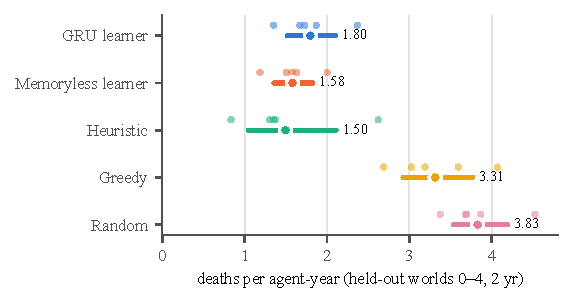
\includegraphics[width=\linewidth]{fig_mortality.pdf}\caption{mortality, mean and 95\% CI; small dots are worlds}\end{subfigure}\hfill
\begin{subfigure}[t]{0.49\linewidth}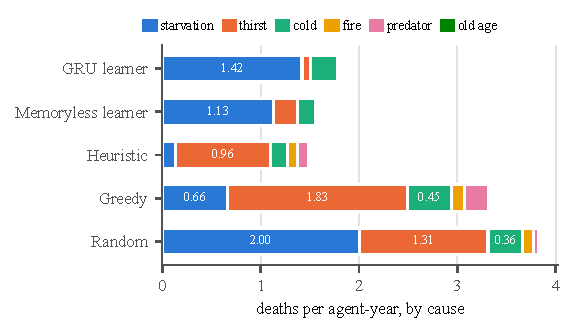
\includegraphics[width=\linewidth]{fig_causes.pdf}\caption{cause-specific death rates}\end{subfigure}
\caption{\textbf{Held-out survival over two years.} (a) Both learners separate from random and greedy, with no
overlap between CIs, but overlap the heuristic. (b) The causes differ completely. The heuristic dies of
\emph{thirst} (0.96 \dpay{}). The learners die of \emph{starvation} (1.42 and 1.13) and have almost no predator or fire
deaths.}
\label{fig:main}
\end{figure}

Table~\ref{tab:main} and Fig.~\ref{fig:main} give the primary outcome.
\begin{itemize}
\item \textbf{H1 is supported.} Both learners beat random and greedy on every world, with non-overlapping CIs and
$|g|>2.9$.
\item \textbf{H2 is not supported.} Both learners' CIs overlap the heuristic's, and both point estimates are
slightly worse. They beat it on only one of five worlds (world 3).
\end{itemize}
The two learners and the heuristic reach similar totals by completely different routes (Fig.~\ref{fig:main}b):
\begin{itemize}
\item \textbf{Thirst:} 0.09 [0.04, 0.14] (GRU) and 0.24 [0.11, 0.36] (memoryless), against 0.96 [0.62, 1.31] for the
heuristic.
\item \textbf{Predators and fire:} 0.006--0.011 for the learners, an order of magnitude below the heuristic's
0.11 each.
\item \textbf{Starvation:} 1.42 [1.17, 1.62] and 1.13 [0.96, 1.28] for the learners, against 0.14 for the
heuristic.
\end{itemize}
A survival-only learner with no water-seeking rule thus learned to manage hydration far better than our hand-written
rules, and failed on energy.

\subsection{Memory: fewer thirst deaths, more starvation (H3 mixed)}
GRU agents suffered 2.7$\times$ fewer thirst deaths than memoryless agents ($g=-1.15$), in the predicted direction.
The cause-specific CIs touch, however, so by our rule the difference is not distinguishable at $n=5$. All-cause
mortality was \emph{higher} with memory: the memoryless agent did better on 5/5 worlds ($g=+0.59$). H3 is therefore
\emph{mixed}. The thirst prediction holds directionally, and the ``no worse overall'' clause fails at this budget.
Section~\ref{sec:energy} offers a mechanism.

\subsection{The deficit is a winter deficit (exploratory)}

\begin{figure}[t]
\centering
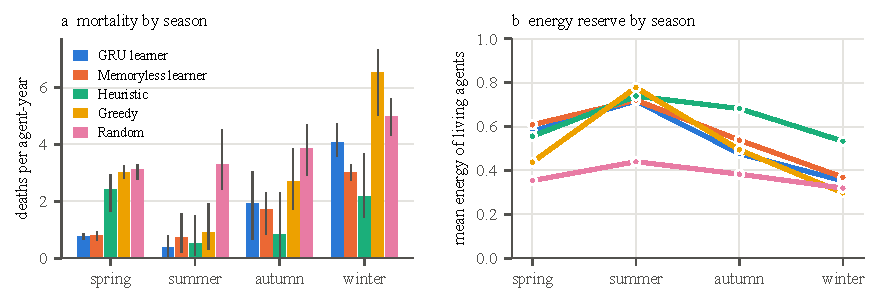
\includegraphics[width=\linewidth]{fig_seasons.pdf}
\caption{\textbf{Mortality and energy by season} (held-out worlds 0--4, 2 yr; bars are means, whiskers the range over
worlds). (a) Learners are the best policies in spring and summer and the worst non-random policies in winter.
The heuristic dies most in spring, when post-winter thirst catches it. (b) The learners enter winter with lower
reserves (0.35--0.37) than the heuristic (0.53).}
\label{fig:seasons}
\end{figure}

\begin{figure}[t]
\centering
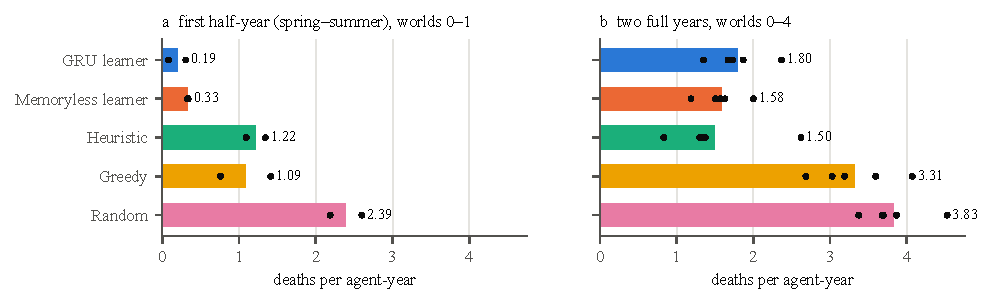
\includegraphics[width=\linewidth]{fig_horizon.pdf}
\caption{\textbf{Evaluation horizon changes the ranking} (exploratory). (a) Over the first half-year after spin-up
(spring--summer; worlds 0--1, the protocol used by the in-training evaluations), learners have 4--6$\times$ lower
mortality than the heuristic. (b) Over two full years they do not. Dots are individual worlds.}
\label{fig:horizon}
\end{figure}

Resolving deaths by season (Fig.~\ref{fig:seasons}) shows that the learners are not uniformly mediocre:
\begin{itemize}
\item \textbf{Spring and summer:} the learners are the \emph{best} policies, at 0.38--0.78 \dpay{}, against
0.50--2.42 for the heuristic.
\item \textbf{Winter:} the GRU learner reaches 4.09 and the memoryless learner 3.03, against 2.16 for the heuristic.
\item \textbf{Energy reserves} fall to 0.35--0.37 in winter, against 0.53 for the heuristic.
\end{itemize}

A shorter evaluation confirms this directly (Fig.~\ref{fig:horizon}). We re-ran all five policies on worlds 0--1 for
half a year, which covers only spring and summer. Over that horizon both learners beat the heuristic: 0.19 and 0.33
against 1.22. Over two years they do not.

This has a methodological consequence. \textbf{Evaluations that do not span a winter would have reported, wrongly, that
the learners beat the hand-written rules.} The in-training mini-evaluations of our replication runs use 0.5-year
horizons. They are useful for tracking progress but must not be used for claims.

A natural hypothesis, which we have not yet tested, is that the effective planning horizon is too short. With
$\gamma=0.995$, credit decays over roughly 200 ticks (1.7 days), while a winter lasts 960 ticks (8 days).
Storing energy in autumn pays off only beyond the discount horizon, which the hand-written ``eat until 0.9'' rule
handles by fiat.

\subsection{Energy economics (exploratory; relevant to preregistered H5)}
\label{sec:energy}

We computed the actual energy gained per meal from the recorded events (each \textsc{eat} event stores the energy
gained) for all 9.8M learner agent-ticks per arm. Table~\ref{tab:energy} gives the result.
\begin{itemize}
\item \textbf{Intake} is $1.31\times10^{-3}$ (GRU) and $1.34\times10^{-3}$ (memoryless) per agent-tick, almost
exactly basal metabolism ($1.3\times10^{-3}$).
\item \textbf{Plants are depleted.} Plants supply 73--74\% of intake, but a plant bite yields only 0.0094 energy on
average, less than a third of the 0.03 nominal value, because cells are grazed down.
\item \textbf{Other sources} are fruit (23--25\%) and meat (2--3\%). Nearly all of the meat is scavenged: the GRU
agents ate 2{,}692 meat bites but made only 25 small-prey kills and \emph{no} large-prey kills in 2{,}560
agent-years. This is consistent with the preregistered H5 for the replication (at most 1 large kill per 1{,}000
agent-years).
\end{itemize}

A first-order budget adds basal cost, halved while resting, and $9\times10^{-4}$ per move, scaled by terrain, so the
move cost is a lower bound. It explains the arm difference:
\begin{itemize}
\item \textbf{GRU agents} move on 37\% of ticks and rest on 16\%. Their expenditure is $\gtrsim1.52\times10^{-3}$,
a deficit of about $2\times10^{-4}$ per tick.
\item \textbf{Memoryless agents} move on 24\% of ticks and rest on 28\%. Their expenditure is
$\gtrsim1.34\times10^{-3}$, roughly in balance.
\end{itemize}
In winter the memoryless agent rests on 48\% of ticks, against 23\% for the GRU agent (Fig.~\ref{fig:behaviour}a).
The better-surviving learner is the one that \emph{does less}. One plausible reading is that the GRU agent explores
more because its memory makes exploring for water pay off. That would explain both its lower thirst and its higher
starvation, but we have not established it causally.

\begin{table}[t]
\centering\small
\caption{\textbf{Energy budget per agent-tick} from recorded events (held-out worlds 0--4 $\times$ 2 yr). Expenditure
is a first-order lower bound: basal $1.3\times10^{-3}$, halved when resting; moves $9\times10^{-4}$ times the share of
move actions; terrain, snow, body-size and carrying multipliers are omitted.}
\label{tab:energy}
\begin{tabular}{@{}lccccccc@{}}
\toprule
Arm & plant & fruit & meat & intake & move share & rest share & expenditure ($\geq$)\\
\midrule
GRU        & 0.965 & 0.297 & 0.044 & 1.306 & 0.365 & 0.162 & 1.52\\
Memoryless & 0.981 & 0.330 & 0.032 & 1.342 & 0.243 & 0.276 & 1.34\\
\bottomrule
\multicolumn{8}{@{}l}{\footnotesize Energy values $\times10^{-3}$ per agent-tick.}
\end{tabular}
\end{table}

\subsection{What the learners do}

\begin{figure}[t]
\centering
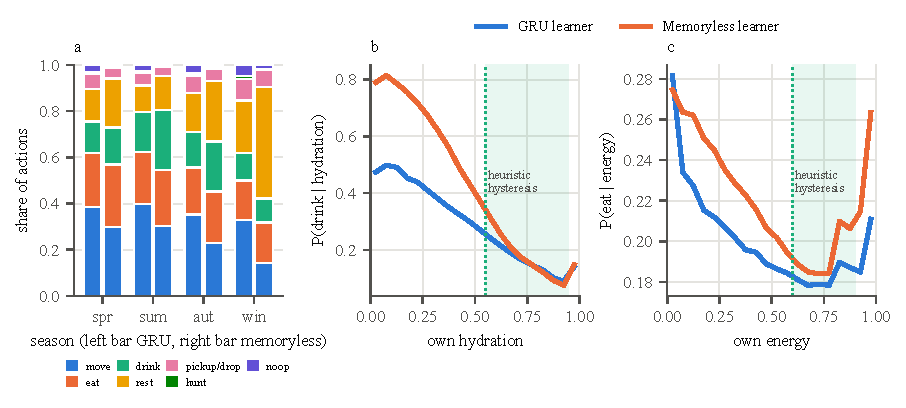
\includegraphics[width=\linewidth]{fig_behaviour.pdf}
\caption{\textbf{Learned behaviour} (all agents, held-out worlds 0--4 $\times$ 2 yr). (a) Action budget by season.
The memoryless agent shifts to resting in winter; the GRU agent keeps moving. (b, c) Learned ``control curves'':
the probability of drinking or eating as a function of the agent's own need. The shaded band is the heuristic's
hysteresis window. Both learners discovered a graded, need-dependent policy without being told the variables'
meaning. The memoryless agent drinks more urgently when dehydrated.}
\label{fig:behaviour}
\end{figure}

Policy entropy falls from 2.40 nats (uniform over 11 actions) to about 1.2--1.3 (Fig.~\ref{fig:training}a).
\begin{itemize}
\item \textbf{Action budget} (GRU): 37\% moves, 21\% eat, 16\% rest, 15\% drink, 7\% pickup/drop and 1\% hunt.
\item \textbf{Hydration} averages 0.88 for GRU and 0.83 for memoryless agents while alive.
\item \textbf{Control curves.} Both learners' probability of drinking falls smoothly with hydration (from 0.5--0.8
near empty to under 0.1 near full), and the probability of eating falls with energy (Fig.~\ref{fig:behaviour}b,c).
This is a graded version of the heuristic's threshold rules, learned from the reward alone.
\end{itemize}

\paragraph{Behavioural inflexibility under drought (exploratory).}
While watching the viewer we noticed an agent repeatedly ``drinking'' at a stream that a drought had dried up. We
quantified this from the recordings. The kernel logs a drink event whenever fresh water or floodwater is adjacent, or
it is raining, so a \textsc{drink} action with no event means no water was in reach.
\begin{itemize}
\item \textbf{During droughts:} 78\% (GRU) and 91\% (memoryless) of drink actions are futile.
\item \textbf{Outside droughts:} 30\% and 37\%.
\end{itemize}
Learned policies key drinking to places and body state, but do not fully condition on whether water is actually
present. Droughts are rare in training, so this is a natural target for the continual-learning and world-model arms.

\subsection{Training dynamics and the replication in progress}

\begin{figure}[t]
\centering
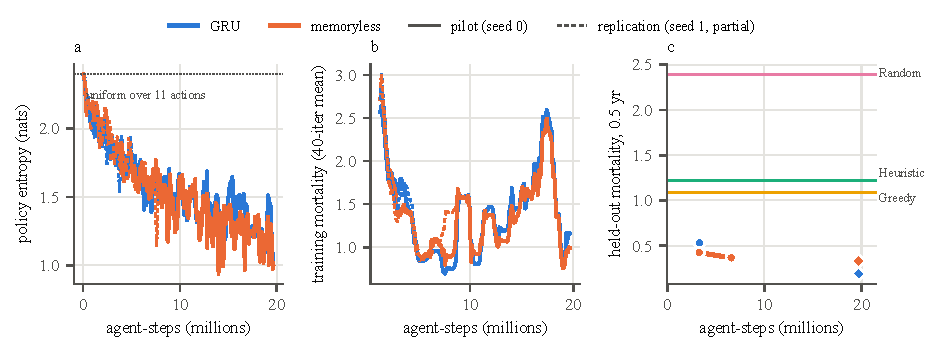
\includegraphics[width=\linewidth]{fig_training.pdf}
\caption{\textbf{Training.} (a) Policy entropy. (b) Training-time mortality (40-iteration moving mean). It oscillates
with the 40-iteration world switch and the seasons and is \emph{not} a usable learning curve. (c) Held-out
mini-evaluations (worlds 0--1, 0.5 yr) of the partial replication runs (circles), the pilots' final checkpoints under
the same protocol (diamonds), and matched baseline levels (lines). Note the half-year caveat of
Fig.~\ref{fig:horizon}.}
\label{fig:training}
\end{figure}

Training-time mortality is dominated by the world schedule and the seasons (Fig.~\ref{fig:training}b), so held-out
evaluation is the only valid learning signal. The preregistered replication trains 3 seeds per arm for 900
iterations (29.5M agent-steps) and evaluates every 100 iterations. It is \emph{paused}, at 154/900 (GRU, seed 1) and
262/900 (memoryless, seed 1). Its first held-out points (0.53 and 0.43 at 3.3M steps; 0.37 at 6.6M for memoryless)
fall well below the half-year baselines, consistent with the pilots (Fig.~\ref{fig:training}c). Its final two-year
evaluation will decide H2$'$ and H3$'$. Separately, an independent re-run of the pilot protocol with the unified learner
(PPOTrainer) reproduced the pilots within their CIs (GRU 1.67, memoryless 1.50 \dpay{}).

\subsection{Internal states, value and social structure (H6, H7 on pilot checkpoints)}
\label{sec:h6h7}
H6 and H7 were preregistered for the replication runs. Here we apply the same analyses, with the same thresholds, to
the pilot checkpoints and their evaluation recordings, so that the pipeline is tested before the decisive data
arrive. The replication remains the confirmatory test. All numbers are in \texttt{stats\_h6\_h7.json}.

\begin{figure}[t]
\centering
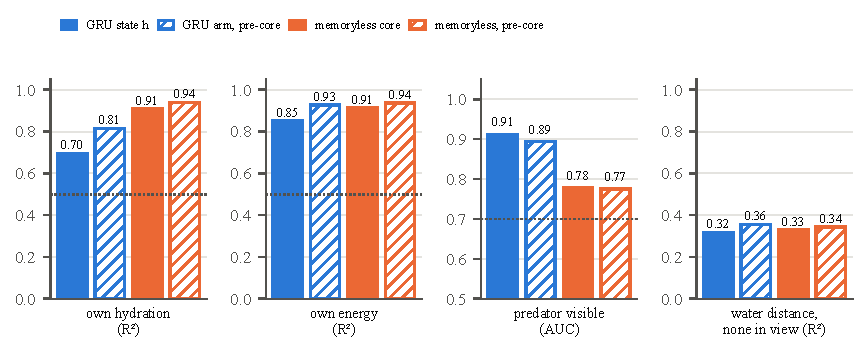
\includegraphics[width=\linewidth]{fig_probes.pdf}
\caption{\textbf{Linear probes} (held-out world 0, first year, 122{,}880 samples per arm; train/test split by agent;
dotted lines are the preregistered thresholds). Solid bars use the core output (GRU state $h$, or the memoryless core);
hatched bars use the same network's pre-core encoding. The right panel is the memory test: decoding log distance to
the nearest fresh water on ticks with \emph{no water in view}. The GRU state does no better than the current encoding.}
\label{fig:probes}
\end{figure}

\paragraph{Probes (H6).}
We replayed held-out world 0 bit-exactly and re-ran each network on the reconstructed observations. Recomputed values
match the recorded ones with correlation $1.000$ and a maximum absolute difference of $1.3\times10^{-6}$. We then fit
ridge and logistic probes with a train/test split by agent (118 test agents).
\begin{itemize}
\item \textbf{GRU state:} hydration $R^2=0.70$, energy $R^2=0.85$, predator-visible AUC $=0.91$, against the
preregistered thresholds of 0.5 and 0.7.
\item \textbf{Memoryless core:} 0.91, 0.91 and 0.78.
\end{itemize}
\textbf{H6 is supported} on the pilots, with two caveats. First, hydration and energy are direct interoceptive inputs,
and the pre-core encodings decode them even better (0.81--0.94), so this is a weak test of anything ``internal''.
Second, a predator is visible on only 0.2--0.4\% of samples. Label-shuffled controls give $R^2\approx0$.

The exploratory memory test asks something sharper. On ticks with no water in view (32--38\% of samples), can the
representation predict how far away the nearest water is? The GRU state reaches $R^2=0.32$, which is \emph{lower} than
its own pre-core encoding (0.36) and no better than the memoryless network (0.33). \textbf{We find no evidence that the
GRU state stores where water is.} Its lower thirst mortality must therefore come from another mechanism, for example
habitually staying closer to rivers (the GRU agents' mean distance to water is 3.4--4.2 cells, against 4.0--4.7 for the
heuristic).

\begin{figure}[t]
\centering
\begin{subfigure}[t]{0.47\linewidth}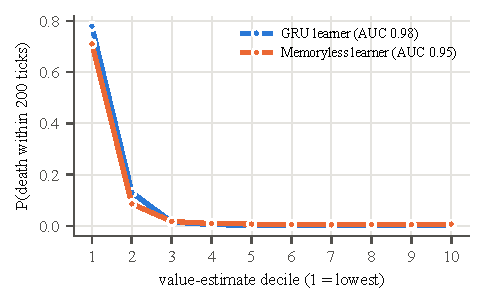
\includegraphics[width=\linewidth]{fig_value.pdf}\caption{value calibration}\end{subfigure}\hfill
\begin{subfigure}[t]{0.51\linewidth}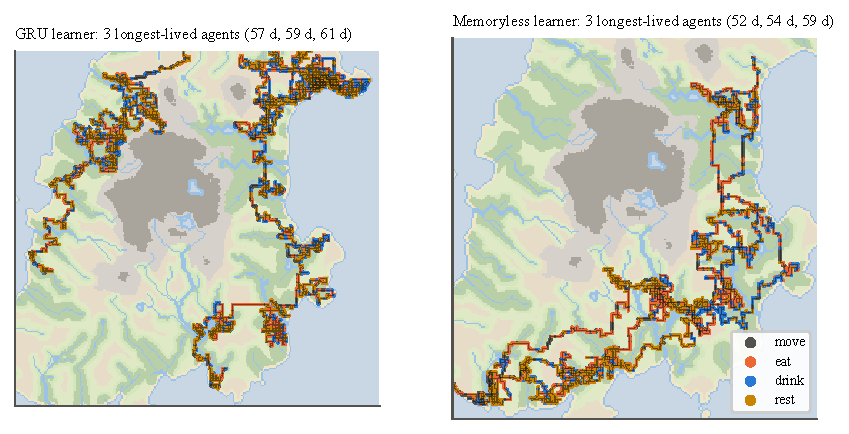
\includegraphics[width=\linewidth]{fig_paths.pdf}\caption{the longest-lived agents on world 0}\end{subfigure}
\caption{\textbf{What the critic knows, and where agents go.} (a) Probability of death within 200 ticks by decile of
the recorded value estimate (worlds 0--4, about 2.4M samples per arm). The lowest decile dies 71--78\% of the time,
against a base rate of 9\%. (b) The three longest-lived agents per arm (52--61 days), coloured by action. Ranges
cover large parts of the island along river corridors.}
\label{fig:value}
\end{figure}

\paragraph{Value calibration (exploratory).}
Across all five held-out worlds, a low recorded value estimate predicts death within 200 ticks with AUC 0.98 (GRU) and
0.95 (memoryless) (Fig.~\ref{fig:value}a). The critic has learned an accurate model of its own mortality risk. This is
a functional correlate useful for analysis, not evidence of anything felt.

\paragraph{Cooperative hunting (H7, part 1).}
The learners attacked large prey 14 times (GRU) and 7 times (memoryless) in 2{,}560 agent-years each, killing none.
\begin{itemize}
\item \textbf{GRU:} one attack episode involved two agents within 6 ticks, against 0.34 expected under the
shuffled-timing null ($p=0.34$).
\item \textbf{Memoryless:} none.
\end{itemize}
The null part of H7 holds, but with almost no statistical power. The baselines teach a methodological lesson. Random
and heuristic agents, which have no social rules at all, ``beat'' the same null: 2 multi-attacker episodes each,
$p=0.004$ and $p=0.04$. Agents drawn to the same herd coincide in time more than shuffled timing allows. \textbf{A
timing-only null is therefore anti-conservative for coordination}, and the replication analysis will use a null that
also preserves spatial co-location, calibrated on baseline agents.

\paragraph{Aggregation (H7, part 2).}
Fig.~\ref{fig:aggregation} compares the Clark--Evans index $R$ \citep{clark1954distance} of the live agents, sampled
daily on worlds 0--4 over 2 years, with two nulls. The first null relocates each agent to a random passable cell at
the same distance from fresh water. The second also matches terrain class and fertility tercile.
\begin{itemize}
\item \textbf{Baselines} sit close to their nulls: ratios 0.95--0.98.
\item \textbf{Learners} are markedly more clustered: 0.77 [0.76, 0.77] (GRU) and 0.82 [0.81, 0.83] (memoryless)
under the water null, and 0.81 and 0.86 under the habitat null.
\end{itemize}
So the second clause of H7, that aggregation does not differ from the heuristic once water is controlled, is
\textbf{not supported}.

Is the clustering social? We tested this causally. We re-ran both trained policies on worlds 0--1 with the agent
channel of the grid and all neighbour features set to zero, which makes them \emph{blind to other agents}. Clustering
did not weaken; it \emph{strengthened}, from 0.77 to 0.71 (GRU) and from 0.83 to 0.78 (memoryless). Mortality was
unchanged: 1.74 vs.\ 1.73 and 1.49 vs.\ 1.52 \dpay{}. The learners therefore cluster \emph{despite} seeing each other,
not \emph{because} of it; if anything, seeing others slightly disperses them. Two non-social explanations remain
open: a shared policy responding identically to dynamic resources that the static nulls ignore (grazed plant patches,
fruiting trees), and synchronised resting sites. \textbf{We do not count this clustering as emergent social
structure.} Without the ablation, it would have been easy to misreport it as such.

\begin{figure}[t]
\centering
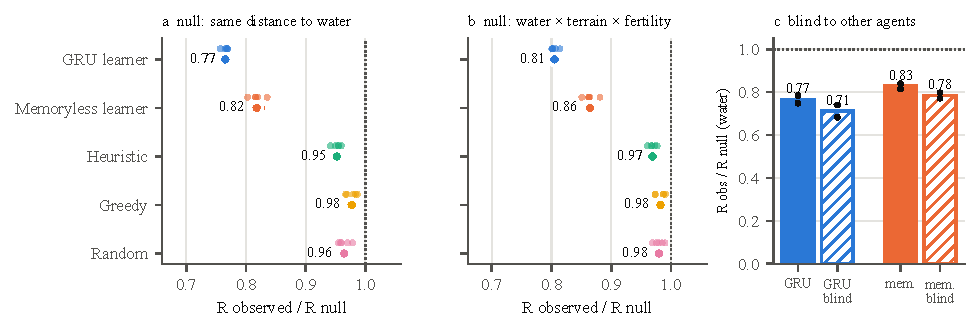
\includegraphics[width=\linewidth]{fig_aggregation.pdf}
\caption{\textbf{Aggregation and its cause.} (a, b) Clark--Evans $R$ relative to two nulls (mean and 95\% CI over
worlds 0--4; small dots are worlds; $<1$ means more clustered than the null). Learners cluster beyond water and
habitat, while the baselines do not. (c) Blinding the trained policies to other agents (agent channel and neighbour
features zeroed; worlds 0--1, 1 yr) does not remove the clustering; it increases it. The clustering is not mediated
by perceiving others.}
\label{fig:aggregation}
\end{figure}

\subsection{Population density (Stage-1 finding)}
Water-seeking baselines collapse at high density. At 1{,}000 agents on the same map, the heuristic reaches 4.94
\dpay{}, with 96\% of deaths from thirst, which is \emph{worse} than random (3.85). At 256 agents it reaches 1.72. Our
hypothesis is congestion at water, which we have not yet tested. Learners must therefore always be compared with
baselines at the same population size.

% =====================================================================================================
\section{Measuring emergence: framework and preregistered nulls}
\label{sec:measure}

The point of \genesis{} is to measure social structure without having put it there. Table~\ref{tab:metrics} lists
the Stage-3 instruments and Fig.~\ref{fig:emerge} the pipeline. Each has three parts:
\begin{enumerate}
\item an operational definition computable from the flight recorder;
\item a null model that removes the social explanation while preserving ecological confounds;
\item a unit test on synthetic data with planted ground truth.
\end{enumerate}
The onset of a phenomenon is the first sustained exceedance of its null's 95\% band. Its \emph{order} across phenomena
is what will eventually be compared, as a structural analogy only, with a cited human timeline in which every entry is
verified or flagged \texttt{UNVERIFIED}. The comparison uses Kendall's $\tau$ over onset ranks.

\begin{figure}[t]
\centering
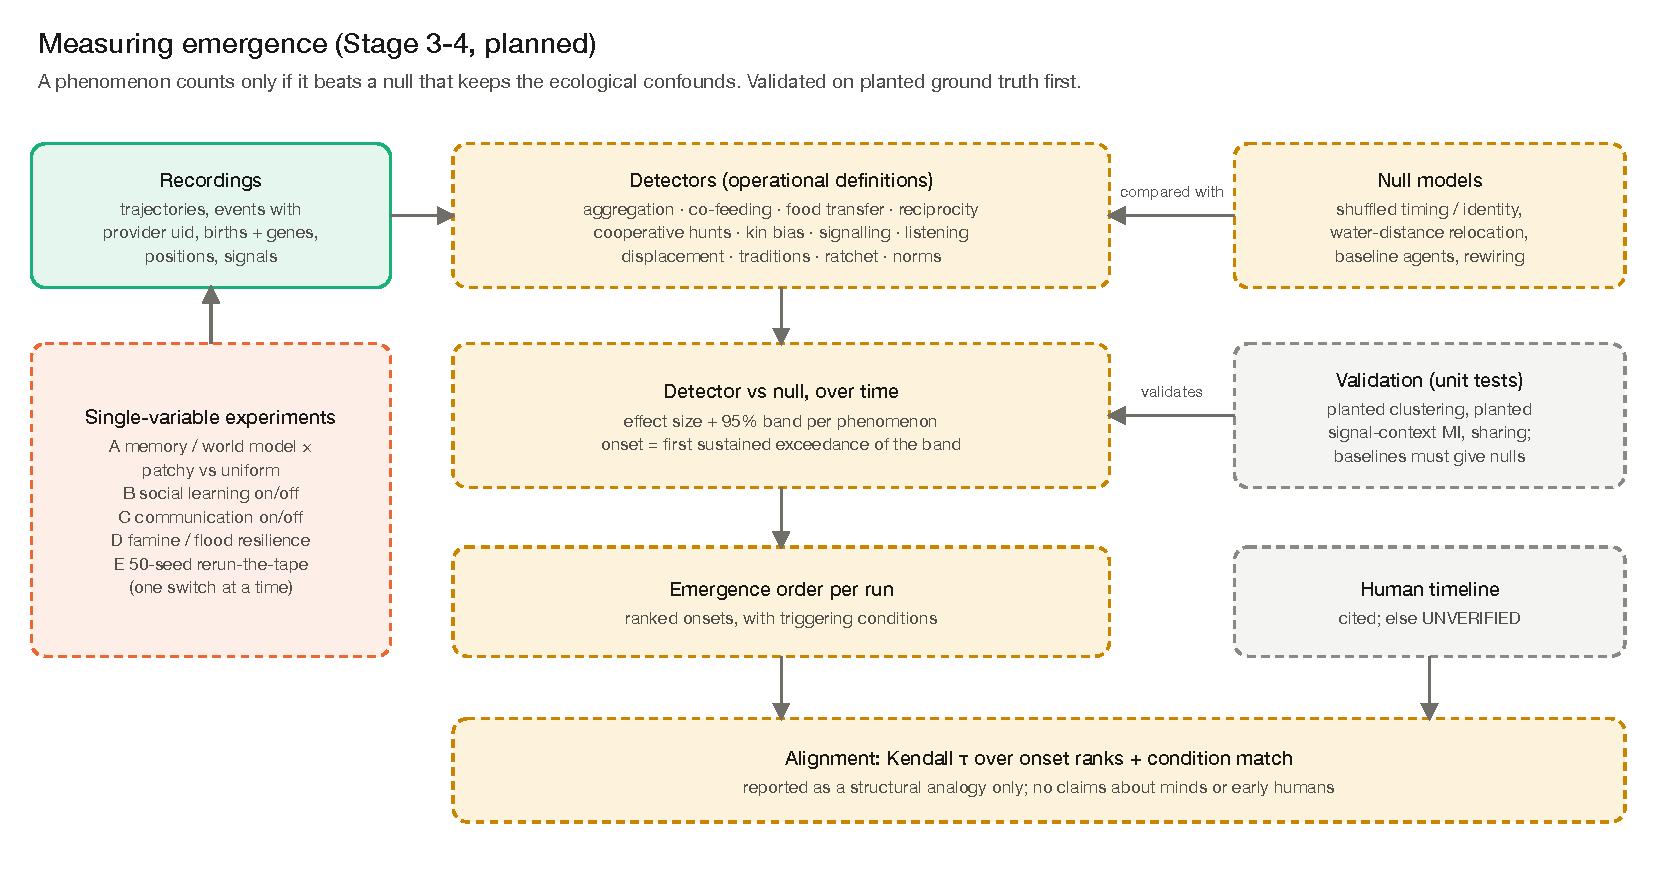
\includegraphics[width=\linewidth]{diagrams/08_emergence_measurement.pdf}
\caption{\textbf{Measuring emergence (planned).} Detectors are computed from the recordings and compared with null models that keep ecological confounds; they are validated on planted ground truth. Onsets give an emergence order, which is compared with a cited human timeline as a structural analogy only.}
\label{fig:emerge}
\end{figure}

\begin{table}[t]
\centering\small
\caption{\textbf{Stage-3 measurement framework} (built: \checkmark; designed and preregistered but not yet run: $\circ$).
All social metrics are reported against both a baseline-agent null and a shuffled null.}
\label{tab:metrics}
\begin{tabularx}{\linewidth}{@{}l X X c@{}}
\toprule
Phenomenon & Operational metric & Null / control & \\
\midrule
Aggregation & Clark--Evans $R$ \citep{clark1954distance}; group-size distribution & water- and habitat-matched relocation; social blinding & \checkmark\\
Co-feeding & meals from carcasses killed by others (provider uid) & carcass-density null & \checkmark\,(count)\\
Food transfer & \textsc{drop} by $A$ $\to$ \textsc{eat}/\textsc{pickup} by $B$ within $k$ ticks & identity shuffle & $\circ$\\
Reciprocity & corr.\ of $A{\to}B$ and $B{\to}A$ transfers & degree-preserving rewiring & $\circ$\\
Cooperative hunt & large-prey attacks with $\geq2$ attackers in 6 ticks & shuffled timing (anti-conservative; \S\ref{sec:h6h7}) & \checkmark\\
Kin bias & transfers/proximity vs.\ genetic similarity & gene-label permutation & $\circ$\\
Signalling & $I(\text{signal};\text{context})$ (positive signalling) & shuffled contexts & $\circ$\\
Listening & causal effect of a heard symbol on action \citep{lowe2019pitfalls} & symbol intervention & $\circ$\\
Displacement & signals predicting out-of-view resources \citep{hockett1960origin} & in-view-only control & $\circ$\\
Traditions & group-specific behaviours not explained by ecology/genes \citep{whiten1999cultures} & ecology-matched groups & $\circ$\\
Ratchet & gen.-$n$ performance with vs.\ without social learning \citep{tennie2009ratchet} & social learning off & $\circ$\\
Norms & strikes conditional on target's sharing history & random targeting & $\circ$\\
Resilience & mortality impact and recovery time after disturbances & matched undisturbed periods & $\circ$\\
Internal states & linear probes \citep{alain2016probes} for hydration, energy, predator & pre-core encoding; shuffled labels & \checkmark\\
Value calibration & AUC of value for death within 200 ticks & base rate & \checkmark\\
\bottomrule
\end{tabularx}
\end{table}

\paragraph{Preregistered for the replication (H5--H7).}
\begin{itemize}
\item \textbf{H5:} starvation stays the leading cause, with at most 1 large-prey kill per 1{,}000 agent-years.
\item \textbf{H6:} a linear probe on the GRU state decodes hydration and energy ($R^2\geq0.5$) and predator presence
(AUC $\geq0.7$). Such results would be functional correlates only, never claims about feelings.
\item \textbf{H7:} multi-attacker large-prey attacks do not exceed a shuffled-timing null, and aggregation does not
differ from the heuristic once distance to water is controlled.
\end{itemize}
Pilot-checkpoint results for H6 and H7 are in \S\ref{sec:h6h7}: H6 is met, cooperative hunting is null, and the
aggregation clause fails for a non-social reason. We expected H7 to hold, a null, in the capability-off setting. Social structure, if any appears, should require the
switches of Table~\ref{tab:switches}.

% =====================================================================================================
\section{Discussion}
\label{sec:discussion}

\paragraph{What the pilots show.}
The survival-only learners are competent in the sense that they beat naive foragers and match a hand-designed
controller. Their competence has a specific shape:
\begin{itemize}
\item they handle water, predators and fire better than our rules do;
\item they handle the energy economy, and especially winter, worse.
\end{itemize}
The world, not the learner, sets this ceiling. Plants are grazed down to about a third of their nominal value, prey
are hard to catch, and large prey require coordination that the agents do not achieve. We will not tune the world to
rescue the learner. If no strategy can generate a surplus, that is itself a property of the ecology to report. The
more interesting question is whether the \emph{only} route to a surplus is cooperative. Two candidates are hunting
large prey together and caching food in autumn, which are exactly the affordances the testbed exposes.

\paragraph{Look-alikes of social structure.}
The pilots already produced two phenomena that a less careful pipeline would have reported as emergent sociality.
First, learners cluster far beyond what water and habitat explain. Second, baseline agents with no social rules
``coordinate'' large-prey attacks beyond a timing null. Neither survives the right control: social blinding for the
first, a baseline-calibrated null for the second. We take this as the main methodological lesson so far. Every
candidate social phenomenon needs a causal ablation of the social channel and a null calibrated on agents that
provably lack the capacity.

\paragraph{Why this matters for emergence claims.}
If cooperation later appears, we need to know whether it appeared because it was the only way out of an energy trap
or because of a capability switch. Seasonal, cause-resolved and energy-resolved accounting of the kind in
\S\ref{sec:results} is therefore part of the measurement apparatus, not a side analysis. The horizon result
(Fig.~\ref{fig:horizon}) shows how easily a protocol choice can reverse a conclusion.

\paragraph{Limitations.}
\begin{itemize}
\item \textbf{Pilot scale.} There is one training seed per arm, so the variance between training runs is unmeasured.
The 3-seed replication is paused part-way.
\item \textbf{Budget.} 19.7M agent-steps is small for a 1.1M-parameter recurrent policy, and memory benefits may
need more training.
\item \textbf{Determinism.} MPS arithmetic is not bit-reproducible. Worlds, sampling and the CPU path are.
\item \textbf{Learner versions.} The pilots were trained with the original \texttt{agents/rppo.py}. It has since
been folded into \texttt{agents/ppo.py} (PPOTrainer), whose defaults are now the pilots' settings. An independent
re-run with PPOTrainer reproduces the pilots within their CIs: 1.67 [1.45, 1.92] (GRU) and 1.50 [1.30, 1.75]
(memoryless) \dpay{} (\texttt{reports/stage2/STAGE2\_REPORT.md}). The pilot checkpoints predate the current
checkpoint format and are loaded by \texttt{pilot\_net.py} in this directory.
\item \textbf{Exploratory analyses.} The seasonal, energy, horizon and drought analyses were not preregistered. The
half-year comparison uses only two worlds. H6 and H7 were preregistered for the replication and are applied here
to pilot checkpoints. Probes use one world, and the blinding ablation uses two worlds and one year.
\item \textbf{Ecology.} Predators hit their immigration floor about 31\% of the time under heuristic pressure.
\item \textbf{Scale of the world.} It is simple compared with any real ecology, and all comparisons to human
prehistory are structural analogies.
\end{itemize}

\paragraph{Broader impact.}
\genesis{} studies how self-interested learners could come to cooperate or conflict, a question relevant to AI
safety and to multi-agent deployment. The system runs on a single laptop, and every run is recorded and exactly
replayable, which supports auditing. We see no direct misuse pathway. The main risk is over-interpretation, such as
reading agent behaviour as evidence about human minds. We address this through restrained language, preregistration
and baselines.

% =====================================================================================================
\section{Roadmap and conclusion}
\label{sec:conclusion}

\genesis{} is designed to be run as a sequence of single-variable experiments:
\begin{itemize}
\item \textbf{A.} Baseline vs.\ memory vs.\ world-model agents (a Dreamer-style latent model \citep{hafner2023dreamerv3}),
crossed with patchy vs.\ uniform resources.
\item \textbf{B.} Social learning on or off across generations: does a cultural ratchet appear?
\item \textbf{C.} Communication on or off: does referential or displaced signalling appear, and do dialects drift?
\item \textbf{D.} Resilience to famine and floods across A--C.
\item \textbf{E.} A 50-seed rerun-the-tape study at reduced scale.
\end{itemize}
Continual-learning probes \citep{kirkpatrick2017ewc,dohare2024plasticity} and lifelong agents with parents and young
come next.

The first study already shows what such a programme needs: held-out worlds, horizons that include the hard season,
non-learning baselines, cause-resolved accounting and preregistered decisions. Under those conditions, survival-only
learners turn out to be good at water, bad at winter, and as yet no better than a page of hand-written rules. We will
report whether anything social emerges with the same rigour, including if the answer is no.

\paragraph{Acknowledgements.} We thank the developers of Numba, PyTorch, three.js and PettingZoo.

{\small
\bibliographystyle{plainnat}
\bibliography{refs}
}

% =====================================================================================================
\clearpage
\appendix
\section*{Appendix}
\addcontentsline{toc}{section}{Appendix}

\section{World details}
\label{app:world}

\begin{table}[h]
\centering\small
\caption{\textbf{Terrain classes.}}
\begin{tabular}{@{}llll@{}}
\toprule
Class & Passable & Move cost & Notes\\
\midrule
Deep water & no & -- & ocean is salt; deep lake cores fresh (drink from shore)\\
Shallow & yes & $\times2$ & rivers, streams, lake rims fresh; ocean shoreline salt\\
Sand, grass, meadow, barren & yes & $\times1$ & fertility differs (meadow highest)\\
Forest & yes & $\times1.25$ & wood, most fruit trees, $+2\,^\circ$C, two cells block sight\\
Rock & yes & $\times1.6$ & stone; hills\\
Mountain & no & -- & blocks line of sight\\
Cave & yes & $\times1$ & shelter: $+10\,^\circ$C, rain cover, predators never enter\\
\bottomrule
\end{tabular}
\end{table}

\begin{table}[h]
\centering\small
\caption{\textbf{Key ecological parameters} (\texttt{configs/default.yaml}).}
\footnotesize\setlength{\tabcolsep}{3pt}\begin{tabular}{@{}ll@{\hspace{1em}}ll@{}}
\toprule
Plant growth rate & 0.0045 /tick & Plant bite / energy per biomass & 0.25 / 0.12\\
Season growth (Sp/Su/Au/Wi) & 1.2 / 1.0 / 0.55 / 0.05 & Grazing floor & 10\% of capacity\\
Fruit energy / max per tree & 0.15 / 6 & Meat bite / energy per unit & 0.2 / 1.0\\
Drink amount / rain drink & 0.22 / 0.006 & Hydration cost & 0.0016 /tick\\
Basal / move cost & 0.0013 / 0.0009 & Rest factor (basal) & 0.5\\
Small prey: kill p / carcass & 0.6 / 0.30 & Large prey: attackers / window & $\geq2$ / 6 ticks\\
Predator: attack p / damage & 0.4 / 0.08 & Fauna torpor below 5\,$^\circ$C & metabolism $\times0.2$\\
Fire ignition / spread & 0.04 /day / 0.22 & Famine probability & 0.08 /year\\
Drought (summer) & 0.06 /day, 6--14 d & Cold snap (winter) & 0.05 /day, 3--7 d, $-10\,^\circ$C\\
\bottomrule
\end{tabular}
\end{table}

\begin{figure}[h]
\centering
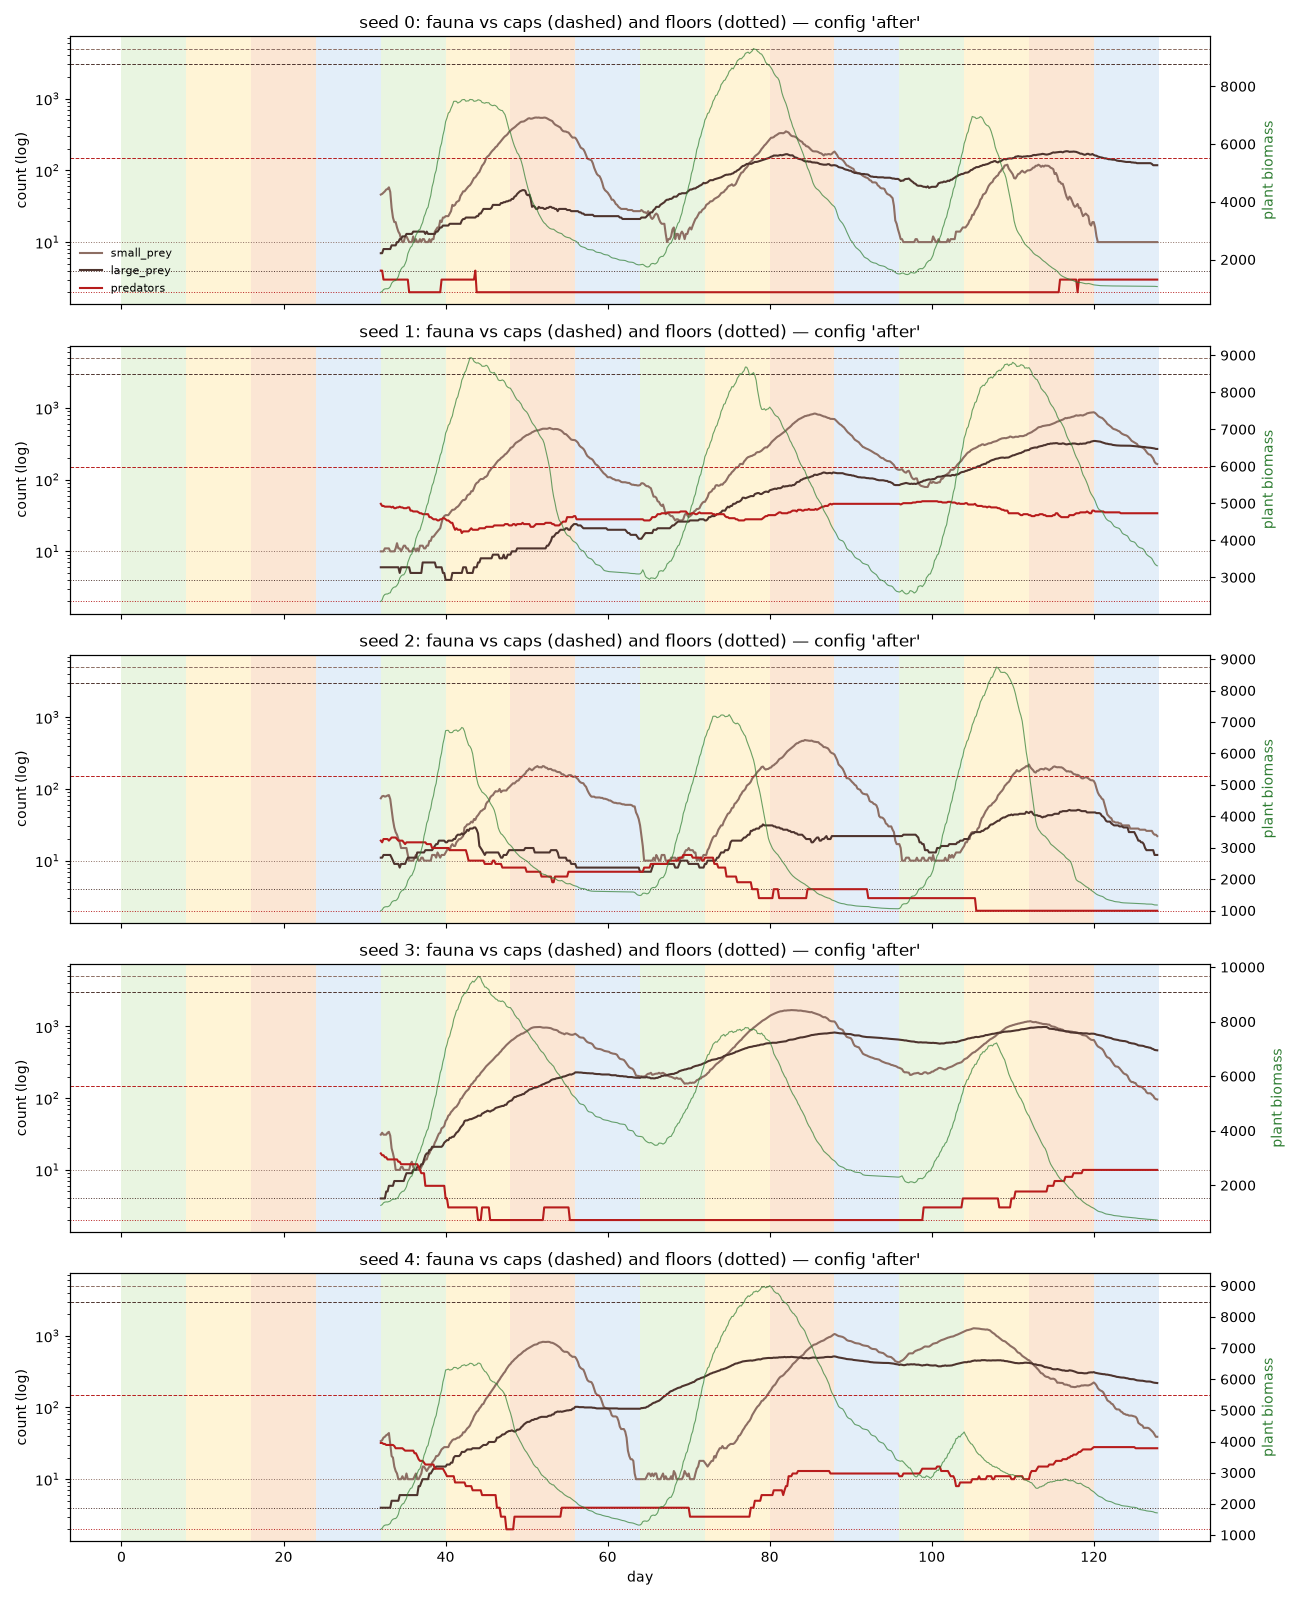
\includegraphics[width=\linewidth]{assets/fig9_fauna_after.png}
\caption{\textbf{Food-limited fauna} (Stage 1.1). Populations are regulated by food, torpor and seasonal breeding,
not by caps, which bind 0\% of the time.}
\end{figure}

\begin{figure}[h]
\centering
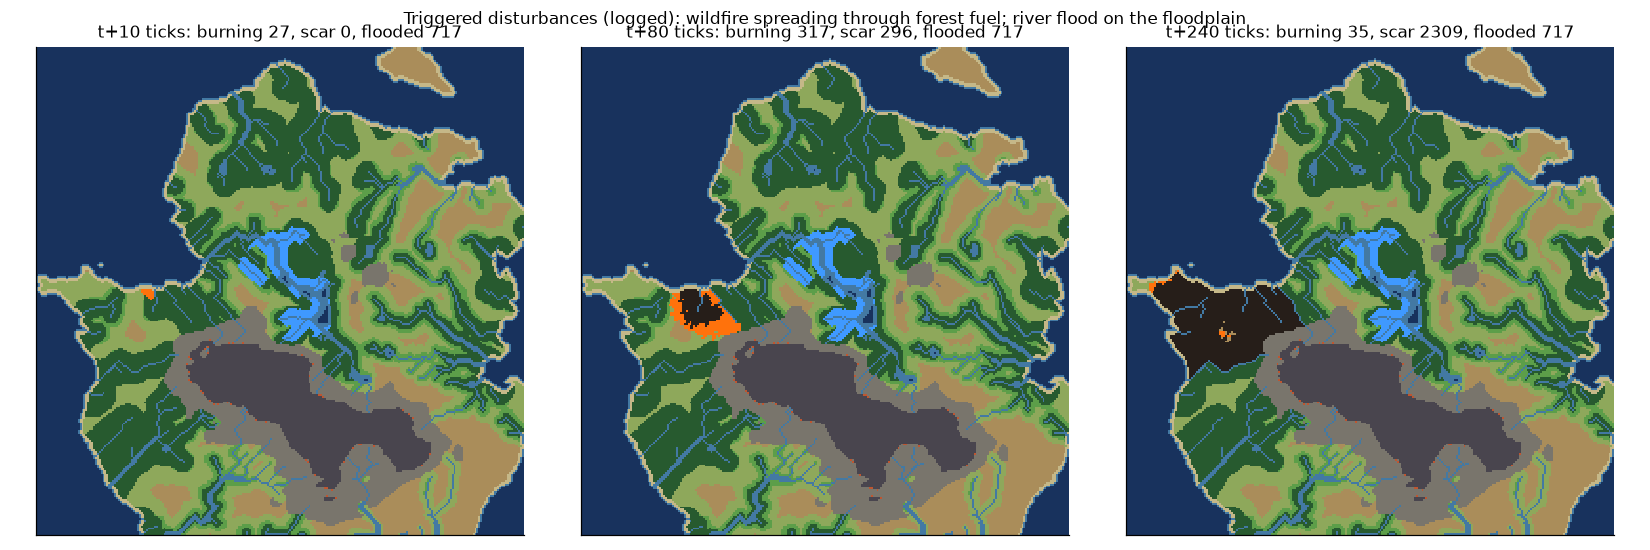
\includegraphics[width=\linewidth]{assets/fig8_disturbances.png}
\caption{\textbf{Disturbances}: wildfire spread and burn scars, spring floods, drought-dried streams and snow.}
\end{figure}

\begin{figure}[t]
\centering
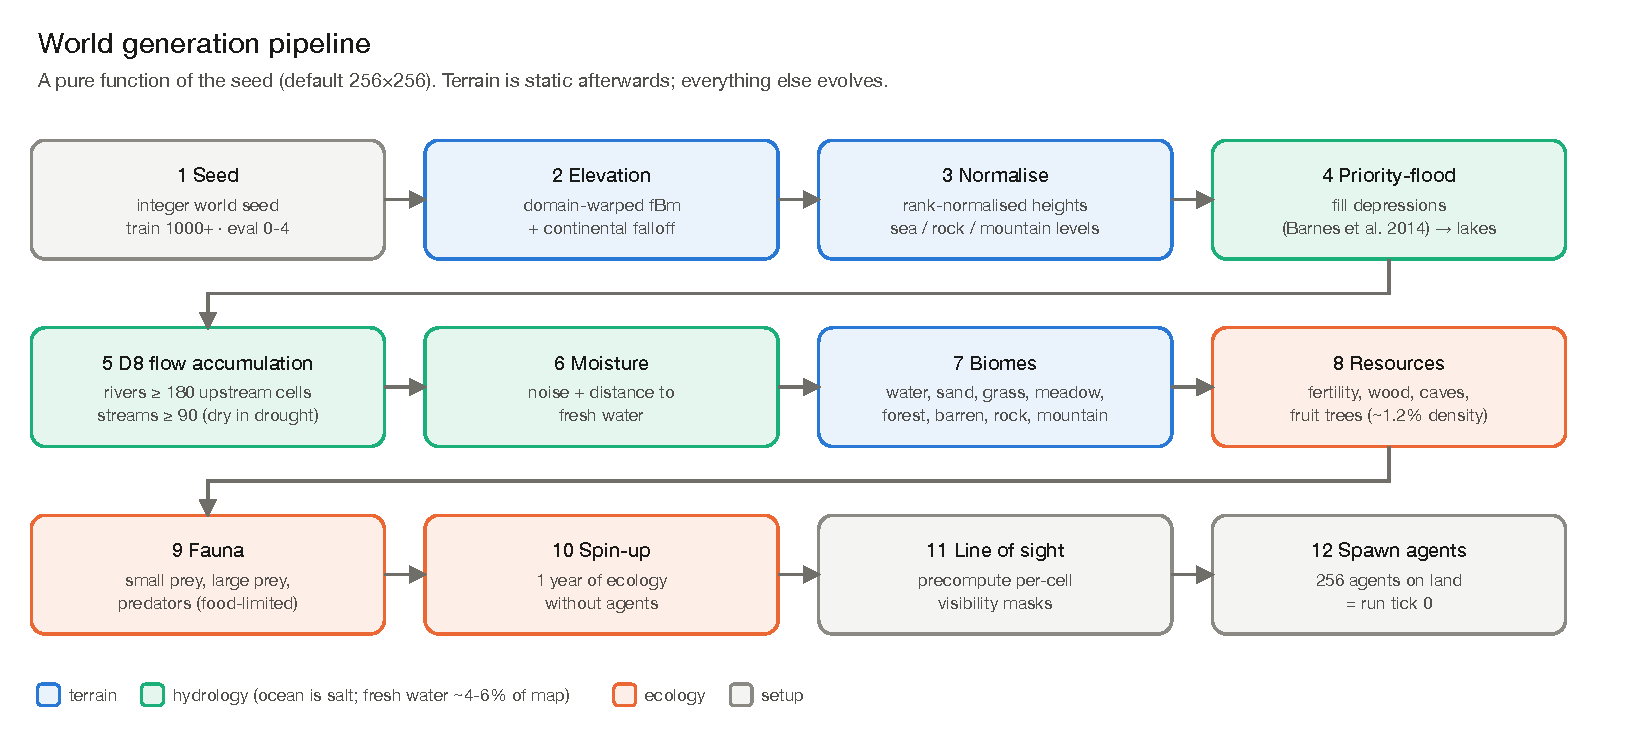
\includegraphics[width=\linewidth]{diagrams/02_world_generation.pdf}
\caption{\textbf{World generation.} The world is a pure function of the seed. Terrain is static afterwards, which is what allows the line-of-sight masks to be precomputed.}
\label{fig:worldgen}
\end{figure}

\begin{figure}[t]
\centering
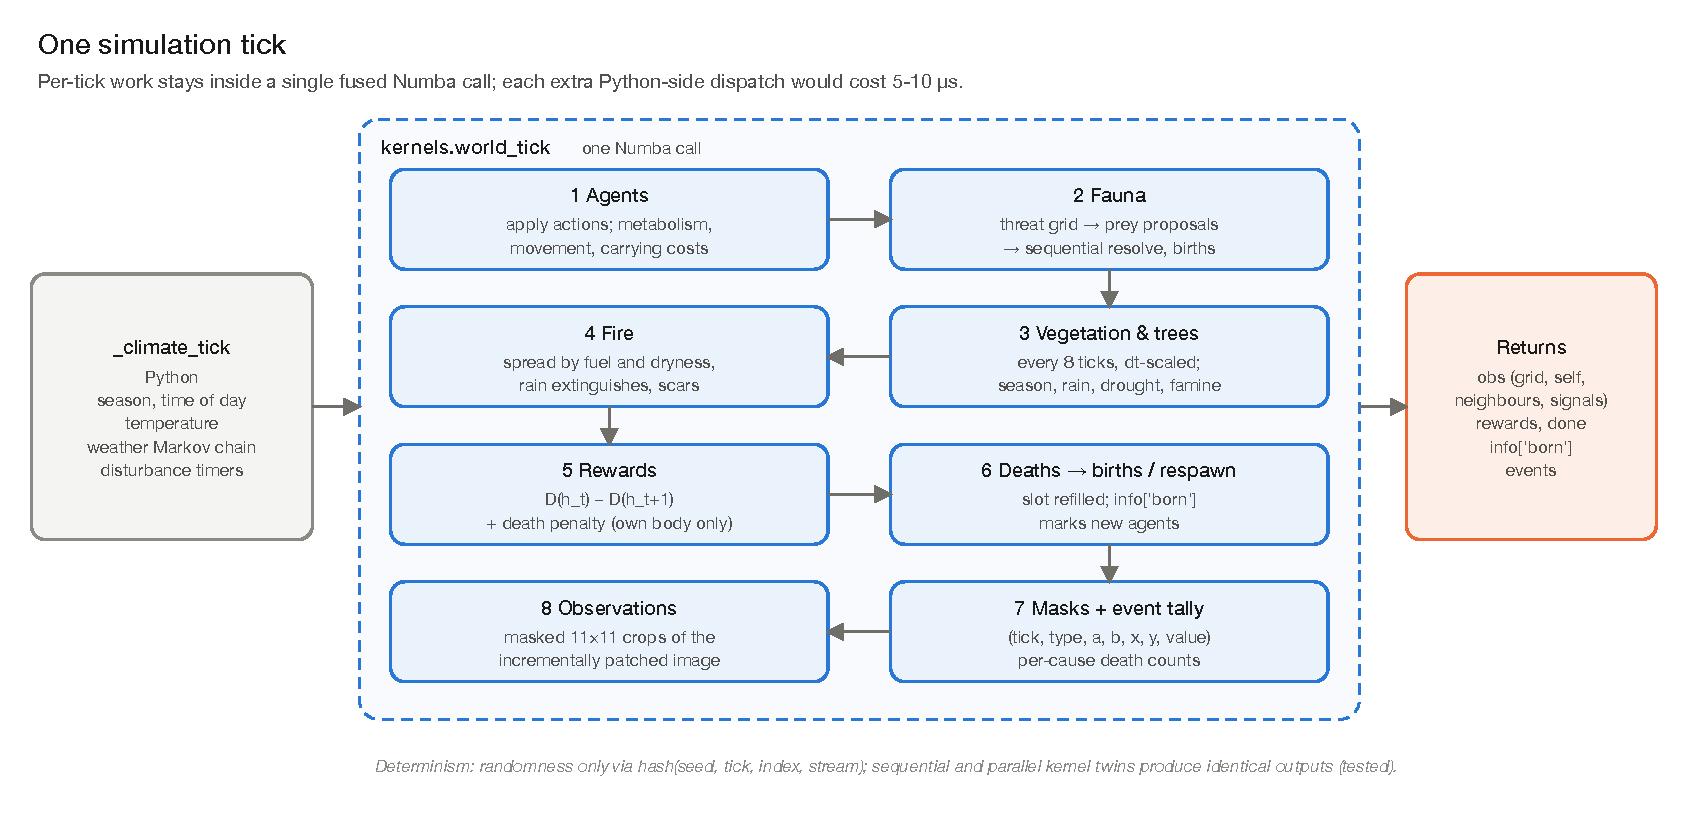
\includegraphics[width=\linewidth]{diagrams/03_world_tick.pdf}
\caption{\textbf{One simulation tick.} A Python climate update followed by one fused Numba call that performs all per-tick work in a fixed order.}
\label{fig:tick}
\end{figure}

\begin{figure}[t]
\centering
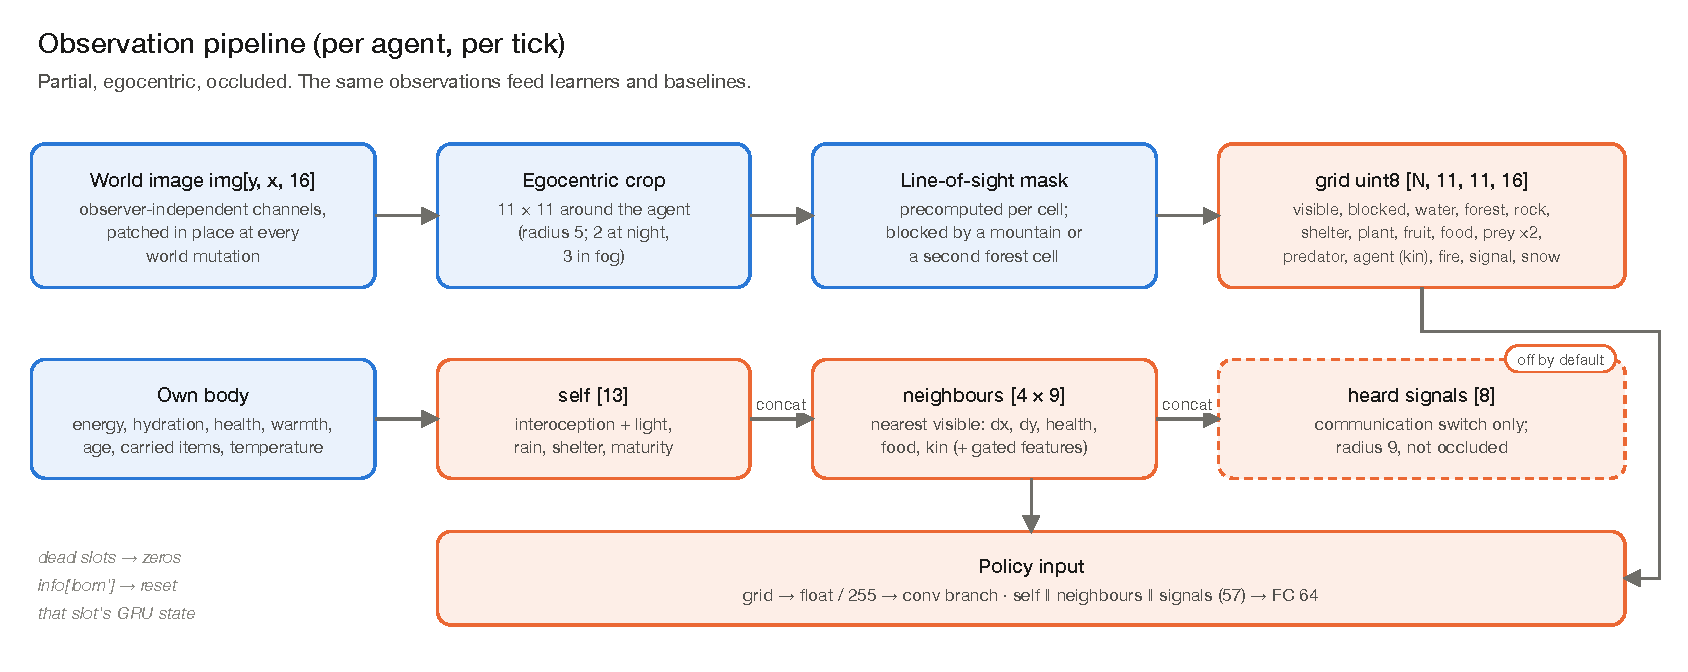
\includegraphics[width=\linewidth]{diagrams/04_observation_pipeline.pdf}
\caption{\textbf{Observation pipeline.} Crops of an incrementally maintained world image are masked by precomputed line of sight and combined with interoceptive and neighbour vectors.}
\label{fig:obspipe}
\end{figure}

\section{Observation and network details}
The 13 self features are energy, hydration, health, warmth, age fraction, carried food, carried wood, carried stone,
felt temperature, light, raining, sheltered and maturity. Each of the 4 nearest visible neighbours contributes 9
features: present, $dx$, $dy$, health, carried food, last action, share rate, strike rate and kin similarity. Last
action is zero unless \texttt{social\_learning} or \texttt{reputation} is on; share and strike rates are zero unless
\texttt{reputation} is on. The grid is cast to float and divided by 255.
The GRU and memoryless arms differ only in the core layer.

\section{Engineering for exact reproducibility}
\begin{itemize}
\item \textbf{Bit-identical runs.} \texttt{test\_full\_run\_bit\_reproducible} asserts that two runs with the same
seed produce identical trajectory hashes, and that different seeds differ.
\item \textbf{Sequential/parallel twins.} Kernels that run sequentially for small workloads (macOS thread launch
costs about 60\,$\mu$s) have parallel twins whose outputs are tested to be identical.
\item \textbf{Flight recorder.} \texttt{sim/recorder.py} stores, for every agent and every tick, the state the agent
acted from, together with its action, reward, death and cause. It also stores learner internals (value, action
probabilities, log-probability), every animal's state, world totals, events, births with genes, and every manual
intervention.
\item \textbf{Replay.} \texttt{analysis.trajectories.replay} re-simulates a recording and checks every agent at every
tick bit-exactly, so observations need not be stored (about 2\,KB per agent per tick otherwise).
\item \textbf{Size.} About 63\,MB per simulated year at 256 agents.
\end{itemize}
The suite has 55 tests, including reward purity, world rules, the PettingZoo API, observation-image drift,
twin agreement, replay and a deterministic end-to-end training loop.

\section{Live viewer}
\label{app:viewer}
A Python aiohttp server runs the simulator in a background thread and streams binary frames over a WebSocket. A three.js client renders a perspective ``diorama'' of the world, with weather, seasons, a day/night
cycle, articulated agents, an inspector showing a selected learner's value estimate and action probabilities,
overlays and a measured-only dashboard. Experiment controls (speed, fire, flood, drought, cold snap, famine,
restart) are applied between ticks and logged, so speed never changes results. Sessions longer than one simulated day
append a summary to the agent log.

\begin{figure}[h]
\centering
\begin{subfigure}[t]{0.49\linewidth}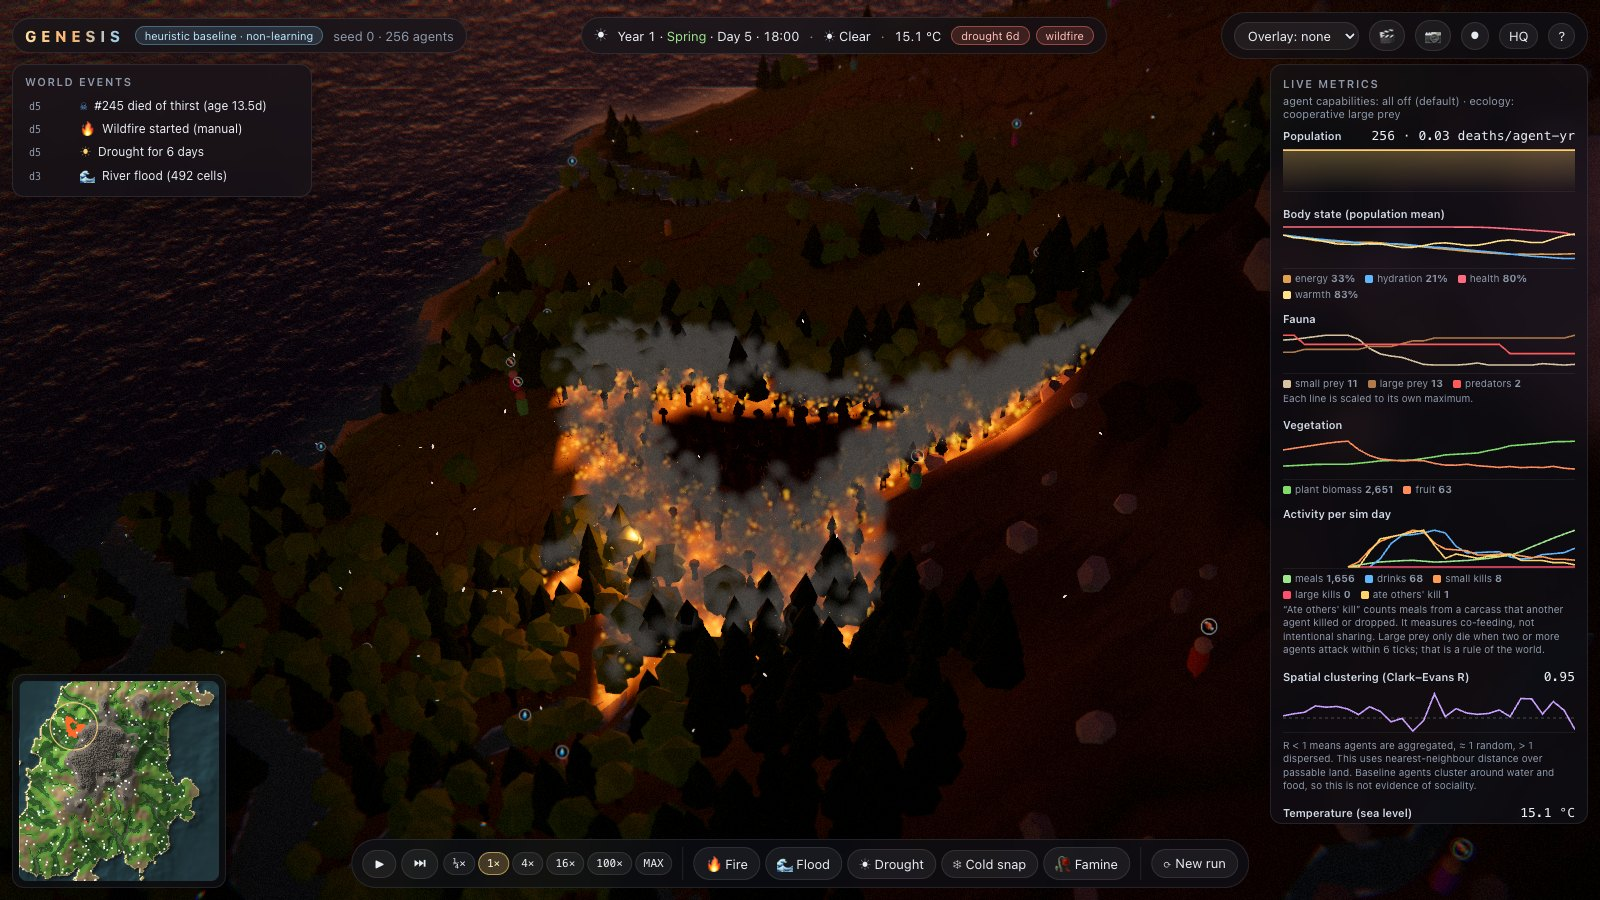
\includegraphics[width=\linewidth]{assets/05_wildfire.jpg}\caption{triggered wildfire}\end{subfigure}\hfill
\begin{subfigure}[t]{0.49\linewidth}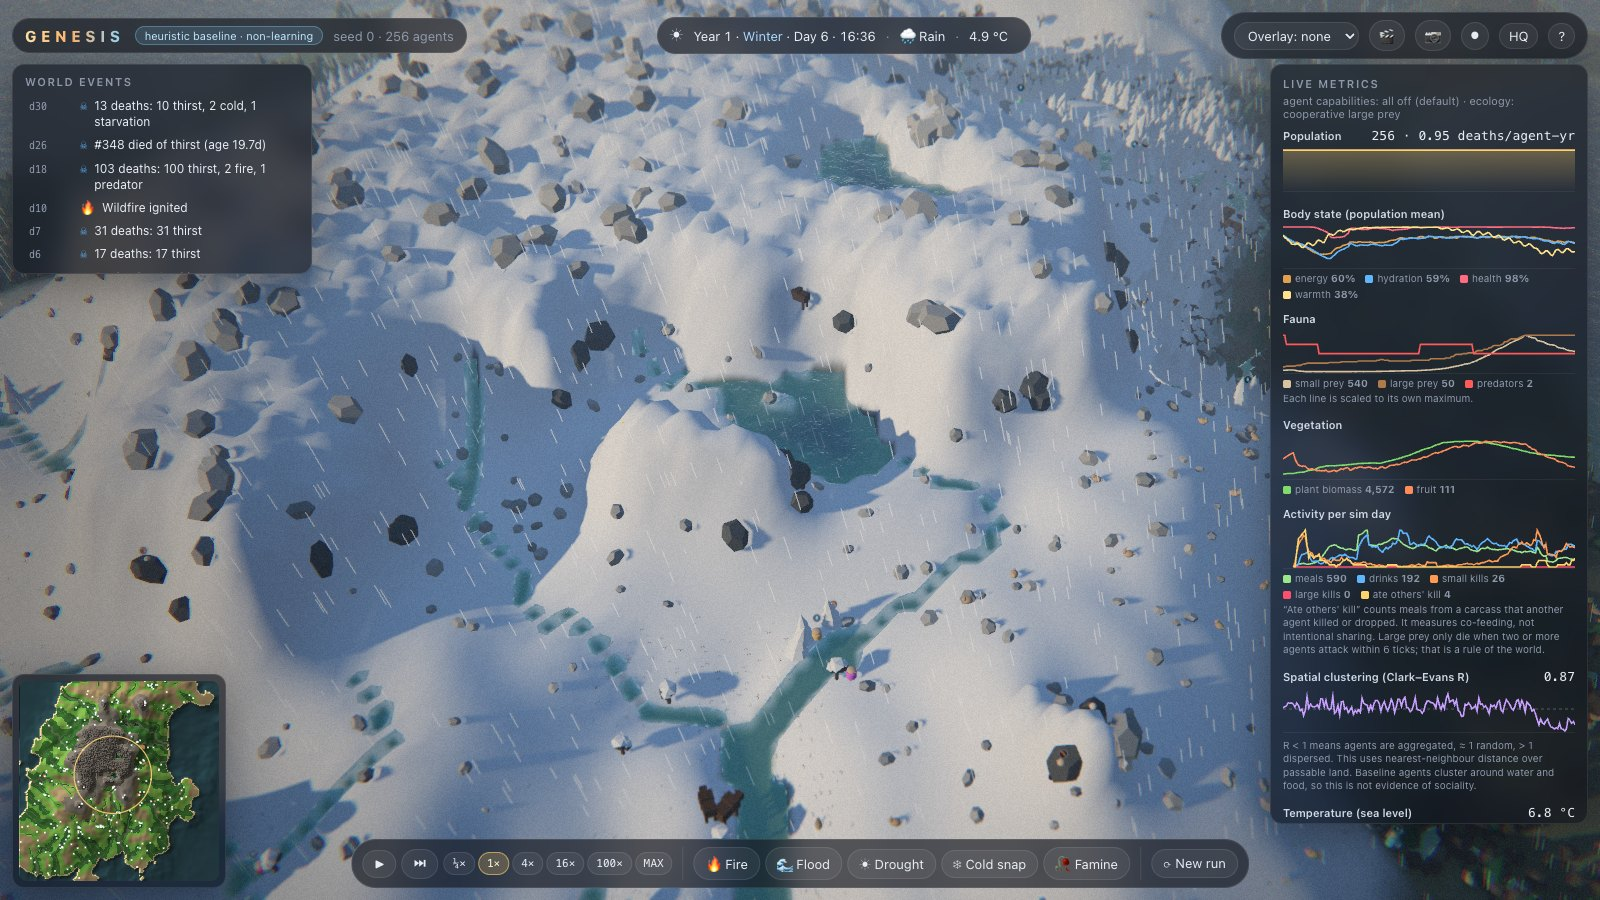
\includegraphics[width=\linewidth]{assets/09_winter.jpg}\caption{winter}\end{subfigure}\\[4pt]
\begin{subfigure}[t]{0.98\linewidth}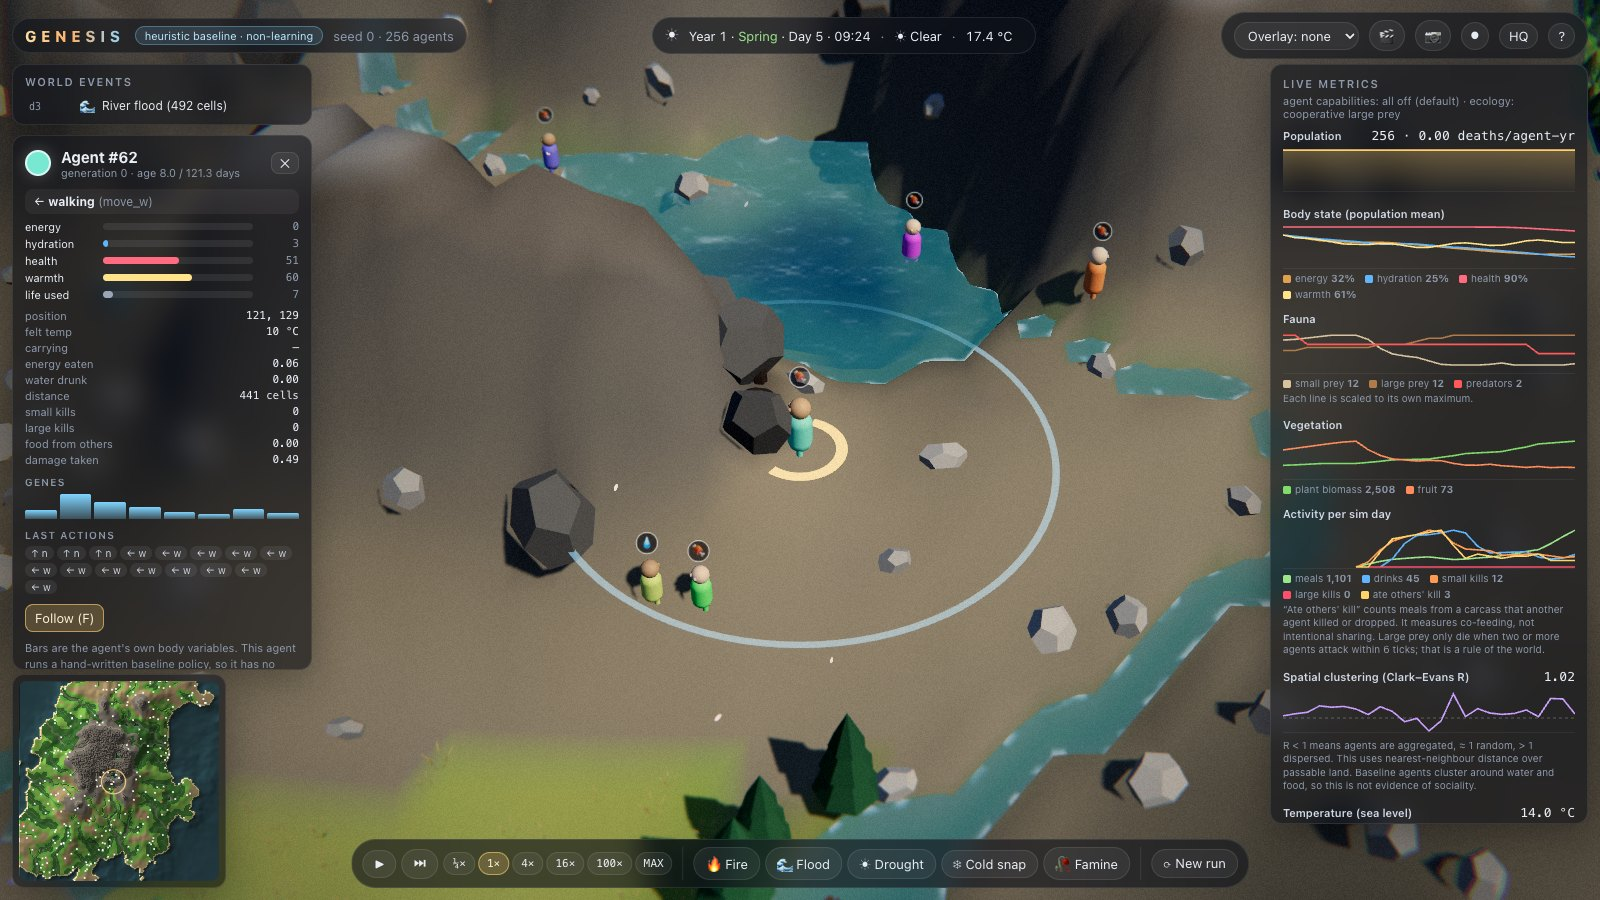
\includegraphics[width=\linewidth]{assets/03_inspector_follow.jpg}\caption{inspector following one agent}\end{subfigure}
\caption{\textbf{Viewer screenshots.} Disturbance controls trigger the same logged \texttt{trigger\_*} methods the
experiments use.}
\end{figure}

\section{Per-world results}
\begin{table}[h]
\centering\small
\caption{\textbf{Deaths per agent-year on each held-out world} (2 yr, 256 agents).}
\begin{tabular}{@{}lccccc@{}}
\toprule
Policy & world 0 & world 1 & world 2 & world 3 & world 4\\
\midrule
Random & 3.69 & 3.87 & 4.53 & 3.37 & 3.68\\
Greedy & 3.59 & 3.19 & 4.07 & 3.03 & 2.69\\
Heuristic & 1.37 & 1.35 & 2.62 & 0.83 & 1.30\\
GRU learner & 1.73 & 1.87 & 2.37 & 1.35 & 1.67\\
Memoryless learner & 1.63 & 1.58 & 2.00 & 1.19 & 1.51\\
\bottomrule
\end{tabular}
\end{table}

\begin{table}[h]
\centering\small
\caption{\textbf{Mortality by season} (\dpay{}, mean over worlds 0--4) and \textbf{mean energy of living agents}.}
\begin{tabular}{@{}lcccc@{\hspace{1.5em}}cccc@{}}
\toprule
& \multicolumn{4}{c}{mortality} & \multicolumn{4}{c}{energy}\\
Policy & Sp & Su & Au & Wi & Sp & Su & Au & Wi\\
\midrule
GRU & 0.76 & 0.38 & 1.93 & 4.09 & 0.58 & 0.72 & 0.48 & 0.35\\
Memoryless & 0.78 & 0.73 & 1.71 & 3.03 & 0.61 & 0.72 & 0.54 & 0.37\\
Heuristic & 2.42 & 0.50 & 0.83 & 2.16 & 0.56 & 0.74 & 0.68 & 0.53\\
Greedy & 3.03 & 0.92 & 2.70 & 6.55 & 0.44 & 0.78 & 0.49 & 0.30\\
Random & 3.10 & 3.28 & 3.87 & 4.97 & 0.35 & 0.44 & 0.38 & 0.32\\
\bottomrule
\end{tabular}
\end{table}

\begin{table}[h]
\centering\small
\caption{\textbf{Population-density sweep} (baselines, 3 seeds $\times$ 1 yr): \dpay{} (thirst share).}
\begin{tabular}{@{}lccc@{}}
\toprule
Policy & 256 agents & 512 agents & 1{,}000 agents\\
\midrule
Random & 3.61 (0.38) & 3.25 (0.33) & 3.85 (0.33)\\
Greedy & 3.61 (0.49) & 3.91 (0.71) & 5.50 (0.78)\\
Heuristic & 1.72 (0.56) & 1.64 (0.86) & 4.94 (0.96)\\
\bottomrule
\end{tabular}
\end{table}

\section{Reproducibility}
\label{app:repro}
\begin{itemize}
\item \textbf{Code.} \url{https://github.com/HeetRanpura/Genesis}. Pilot checkpoints were trained at commits
\texttt{c5ea9ff} (GRU) and \texttt{50143db} (memoryless) and evaluated at \texttt{e1d919e}. The analysis scripts
in \texttt{reports/stage2/pilot\_preprint/} run on current \texttt{main}.
\item \textbf{Software.} Python 3.11, PyTorch 2.14.1 (MPS), Numba 0.68.0, NumPy 2.4.6.
\item \textbf{Hardware.} Learners ran on a MacBook Pro (M3 Pro, 11 cores, 18\,GB). Engine benchmarks ran on a fanless
MacBook Air (M4). Throughput is never compared across machines.
\item \textbf{Seeds.} Training worlds are seeds 1000+ (one new world every 40 iterations). Evaluation worlds are
0--4. The training seeds are 0 (pilots) and 1--3 (replication).
\end{itemize}
{\footnotesize
\begin{verbatim}
make setup && make test                       # environment + tests
.venv/bin/python experiments/run_baselines.py --seeds 5 --years 2
# pilots: trained/evaluated with the original rppo scripts (c5ea9ff, 50143db,
#         e1d919e); today's learner: make train NAME=gru_s0 / make eval NAME=...
.venv/bin/python reports/stage2/pilot_preprint/make_figures.py   # every figure + stats.json
.venv/bin/python reports/stage2/pilot_preprint/analysis_h6_h7.py  # probes, value, hunts, paths
.venv/bin/python reports/stage2/pilot_preprint/aggregation_strict.py  # water + habitat nulls
.venv/bin/python reports/stage2/pilot_preprint/blind_ablation.py  # social blinding
make viewer POLICY=ppo:gru_s0                 # live viewer, http://localhost:8787
\end{verbatim}
}
\begin{itemize}
\item \textbf{Run directories.} Each run directory contains the resolved config, a manifest (git commit, versions),
\texttt{metrics.csv}, \texttt{events.npy} and a \texttt{trajectory/} directory of compressed 480-tick chunks with a
start-state hash. Replay of an older recording fails loudly if the engine's dynamics have changed since.
\item \textbf{Analysis outputs.} \texttt{stats.json} holds every number quoted in \S\ref{sec:results}.
\end{itemize}

\section{Checklist (abridged NeurIPS)}
\begin{itemize}
\item \textbf{Claims match results?} Yes. Negative results (H2, H3) are stated in the abstract.
\item \textbf{Limitations discussed?} Yes, in \S\ref{sec:discussion}.
\item \textbf{Code and data available?} Yes, the repository; run data (several GB) is available on request.
\item \textbf{Training details?} Yes, in Table~\ref{tab:hparams} and Algorithm~\ref{alg:train}.
\item \textbf{Error bars?} Yes: 95\% bootstrap CIs over worlds, plus Hedges' $g$. The unit of replication is stated.
\item \textbf{Compute?} About 50 minutes per pilot run on an M3 Pro (MPS), and about 45\,s per 2-year evaluation
world.
\item \textbf{Preregistration?} Yes, a timestamped file committed before evaluation. Exploratory analyses are
labelled as such.
\item \textbf{Human subjects or sensitive data?} None.
\end{itemize}

\end{document}
